\chapter{Implementation and Deployment}

\section{Introduction}

This chapter presents the implementation and deployment of the TechMart multi-cloud e-commerce platform, demonstrating practical application of both GitOps and Traditional CI/CD methodologies across diverse cloud platforms. The implementation encompasses infrastructure provisioning, service deployment, workflow automation, and operational configuration enabling rigorous empirical comparison between deployment methodologies.

The implementation follows a systematic approach prioritizing both experimental rigor and production-grade operational practices. The deployment architecture demonstrates enterprise-level DevOps practices while maintaining controlled experimental conditions necessary for valid methodology comparison and performance analysis.

The chapter details the progression from infrastructure setup through complete multi-service deployment, showcasing practical challenges and solutions encountered during real-world implementation of sophisticated DevOps methodologies across heterogeneous cloud platforms.

\section{Infrastructure Setup and Deployment}

The infrastructure implementation demonstrates comprehensive cloud-native deployment practices across multiple platforms, each selected for specific characteristics supporting both experimental requirements and production-grade operational capabilities. The implementation prioritizes automation, reproducibility, and security while maintaining flexibility necessary for comparative methodology analysis.

\subsection{Multi-Platform Infrastructure Strategy}

The infrastructure architecture strategically distributes services across multiple cloud providers to create realistic enterprise deployment complexity while enabling controlled methodology comparison. This multi-cloud approach leverages provider-specific capabilities while avoiding vendor lock-in and enabling comprehensive methodology evaluation.

\textbf{Platform Distribution Strategy:}

\begin{table}[H]
\centering
\caption{Multi-Cloud Infrastructure Distribution and Rationale}
\label{tab:infrastructure-distribution}
\begin{tabular}{|p{3cm}|p{3cm}|p{3cm}|p{5cm}|}
\hline
\textbf{Platform} & \textbf{Services} & \textbf{Deployment Method} & \textbf{Strategic Rationale} \\
\hline
Google Kubernetes Engine & User, Order Services & GitOps + ArgoCD & Sophisticated orchestration, declarative management, self-healing capabilities \\
\hline
Heroku Container Stack & Product, Cart Services & Traditional CI/CD & Platform optimization, operational simplicity, direct deployment efficiency \\
\hline
Neon PostgreSQL & User, Order data & Managed relational DB & ACID compliance, complex relationships, transactional integrity \\
\hline
MongoDB Atlas & Product catalog & Managed document DB & Flexible schema, horizontal scaling, advanced search capabilities \\
\hline
Upstash Redis & Cart, Order caching & Managed in-memory DB & High performance, session management, distributed caching \\
\hline
Vercel & Frontend application & Serverless deployment & Global CDN, Git integration, optimal frontend delivery \\
\hline
\end{tabular}
\end{table}

\begin{figure}[H]
\centering
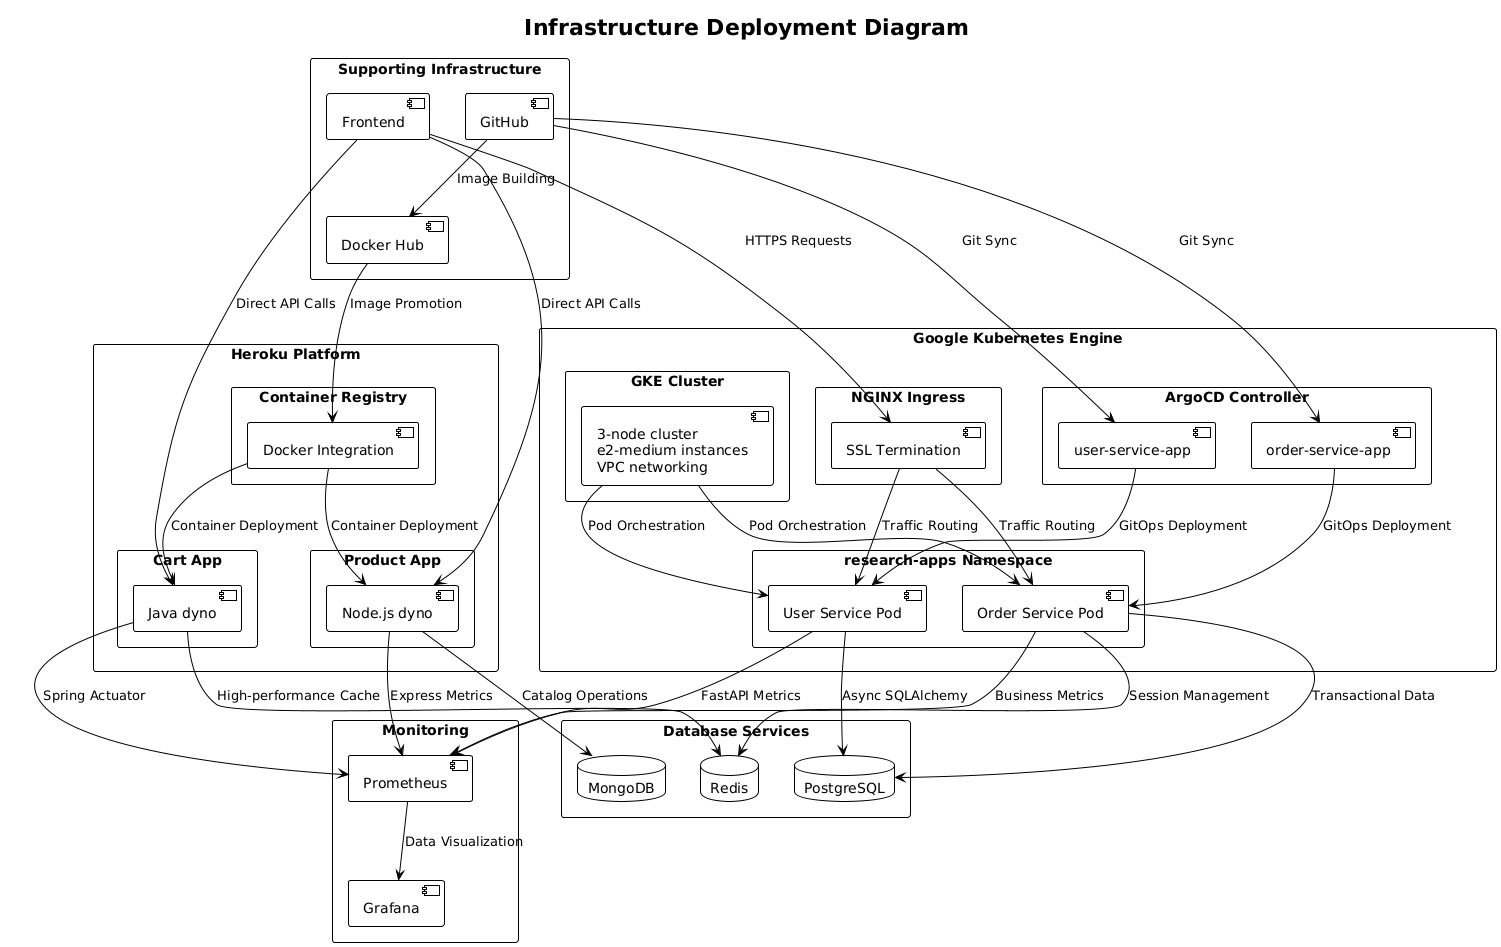
\includegraphics[width=1.0\textwidth]{figures/Infrastructure-Deployment-Diagram.png}
\caption{Infrastructure Deployment Diagram}
\label{fig:infrastructure-deployment-diagram}
\end{figure}

Figure \ref{fig:infrastructure-deployment-diagram} illustrates the multi-platform infrastructure distribution strategy.

\textbf{Infrastructure Selection Criteria:}
\begin{itemize}
\item \textbf{GitOps Platform (GKE):} Required sophisticated orchestration for ArgoCD integration and declarative management
\item \textbf{Traditional CI/CD Platform (Heroku):} Optimal for demonstrating platform-as-a-service benefits and deployment simplicity
\item \textbf{Database Distribution:} Strategic technology selection matching data characteristics and access patterns
\item \textbf{Cost Optimization:} Academic budget constraints (\$300 GCP credits + free tiers) driving strategic service placement
\end{itemize}

\subsection{Google Kubernetes Engine Configuration}

The GKE implementation provides the foundation for GitOps deployment methodology demonstration, showcasing enterprise-grade container orchestration with comprehensive automation and self-healing capabilities.

\subsubsection{Cluster Architecture and Resource Allocation}

\textbf{Cluster Configuration:}
\begin{itemize}
\item \textbf{Node Configuration:} 3-node cluster with e2-medium instances (2 vCPU, 4GB RAM per node)
\item \textbf{Network Architecture:} VPC-native networking with automatic IP allocation and service discovery
\item \textbf{Security Implementation:} Google Cloud IAM integration with RBAC and comprehensive audit logging
\item \textbf{Monitoring Integration:} Google Cloud Monitoring APIs with Prometheus metrics collection
\end{itemize}

\textbf{Research-Specific Configuration:}
\begin{itemize}
\item Dedicated \texttt{research-apps} namespace with resource quotas and network isolation
\item Enhanced logging and metrics collection for experimental data gathering
\item Specialized labeling strategies supporting methodology performance tracking
\item Comprehensive health checking configured for GitOps deployment validation
\end{itemize}

\subsubsection{ArgoCD Installation and GitOps Configuration}

The ArgoCD installation demonstrates comprehensive GitOps workflow automation with enterprise-grade configuration management and deployment orchestration.

\textbf{ArgoCD Deployment Features:}
\begin{itemize}
\item Official Helm chart installation with research-specific customizations
\item GitHub repository integration with \texttt{multicloud-gitops-research} branch as source of truth
\item Automated sync policies with self-healing capabilities and 10-revision rollback history
\item Comprehensive application health checking with dependency management
\end{itemize}

\begin{figure}[H]
\centering
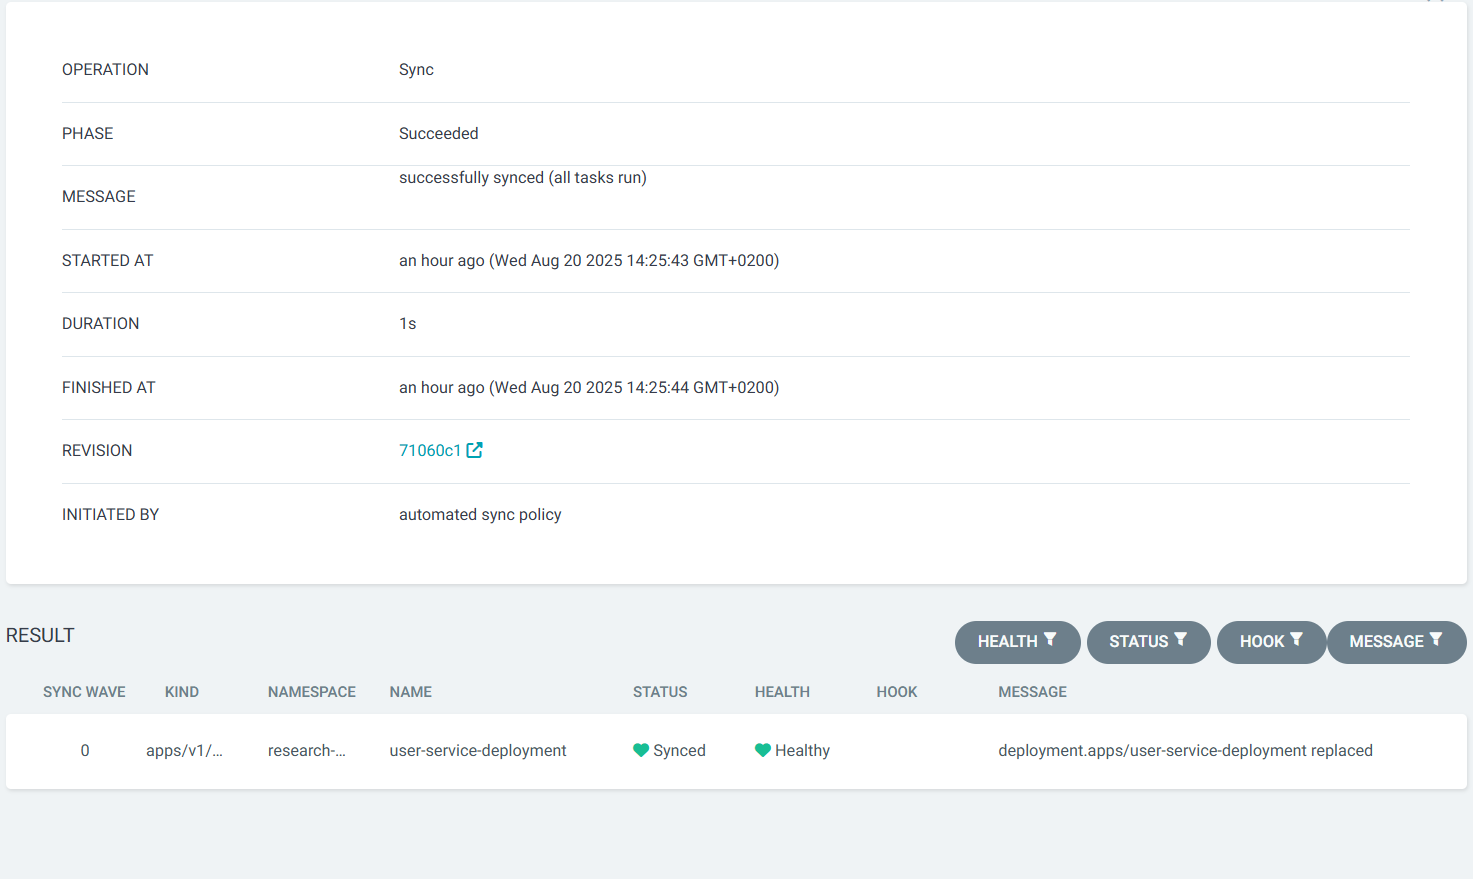
\includegraphics[width=0.9\textwidth]{figures/chapter5/argocd-deployment-sync.png}
\caption{ArgoCD Deployment Synchronization showing GitOps automation in action}
\label{fig:argocd-deployment-sync}
\end{figure}

Figure \ref{fig:argocd-deployment-sync} shows the real-time synchronization process enabled by ArgoCD automation.

\begin{figure}[H]
\centering
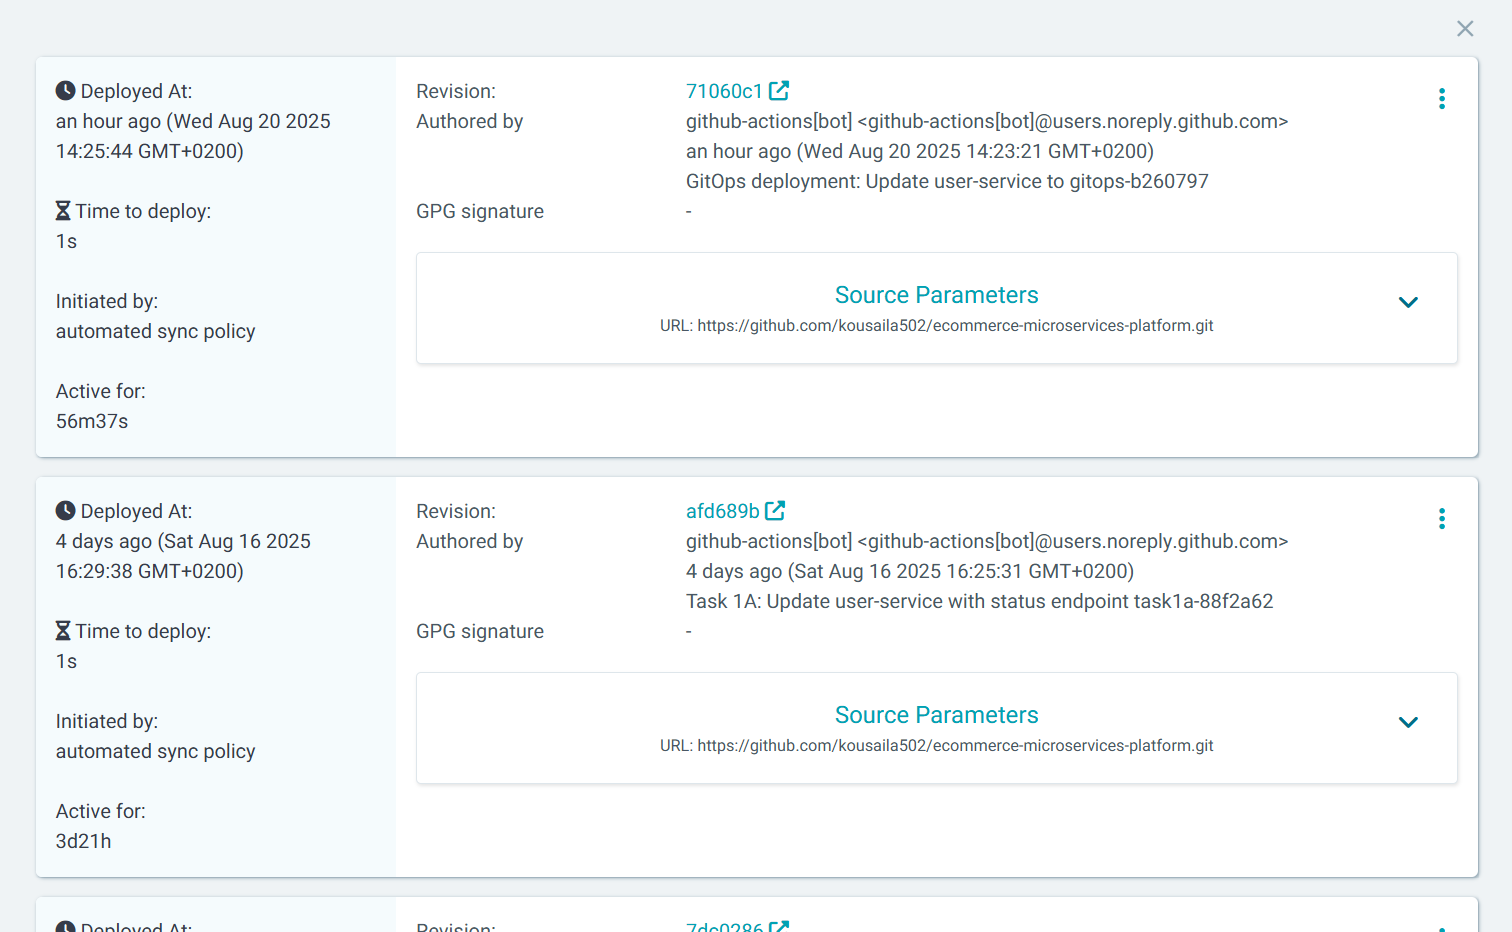
\includegraphics[width=0.9\textwidth]{figures/chapter5/argocd-deployment-history.png}
\caption{ArgoCD Deployment History showing revision tracking and rollback capabilities}
\label{fig:argocd-deployment-history}
\end{figure}

Figure \ref{fig:argocd-deployment-history} demonstrates revision tracking and rollback capabilities in ArgoCD.


\textbf{Kubernetes Resource Management:}
\begin{itemize}
\item NGINX Ingress Controller with Let's Encrypt SSL automation
\item Comprehensive CORS configuration for multi-platform integration
\item Advanced traffic management (connection limiting, rate limiting, load balancing)
\item Rolling update strategies with zero-downtime deployment capabilities
\end{itemize}

\subsection{Heroku Platform Configuration}

The Heroku platform implementation demonstrates mature Platform-as-a-Service deployment patterns with comprehensive operational capabilities and simplified deployment workflows, showcasing Traditional CI/CD methodology advantages.

\subsubsection{Application Provisioning and Platform Integration}



\textbf{Platform-as-a-Service Benefits:}
\begin{itemize}
\item \textbf{Operational Simplicity:} Managed runtime environments with automatic scaling
\item \textbf{Integrated Monitoring:} Built-in application metrics, request tracing, error monitoring
\item \textbf{Security Management:} Automatic SSL certificates, security patching, compliance monitoring
\item \textbf{Cost Efficiency:} Eco dynos for development, standard dynos for production deployment
\end{itemize}

\subsubsection{Container Registry and Deployment Workflow}

\textbf{Heroku Container Stack Integration:}
\begin{itemize}
\item Docker Hub to Heroku Container Registry promotion workflows
\item Automated image validation and security scanning
\item Platform-native release management with health checking
\item Comprehensive deployment tracking and rollback capabilities
\end{itemize}

\textbf{Traditional CI/CD Deployment Characteristics:}
\begin{itemize}
\item Direct platform deployment eliminating orchestration overhead
\item Manual approval gate simulation for enterprise governance patterns
\item Platform-specific optimization benefits (buildpack efficiency, managed services)
\item Comprehensive operational oversight and deployment validation
\end{itemize}

\begin{figure}[H]
\centering
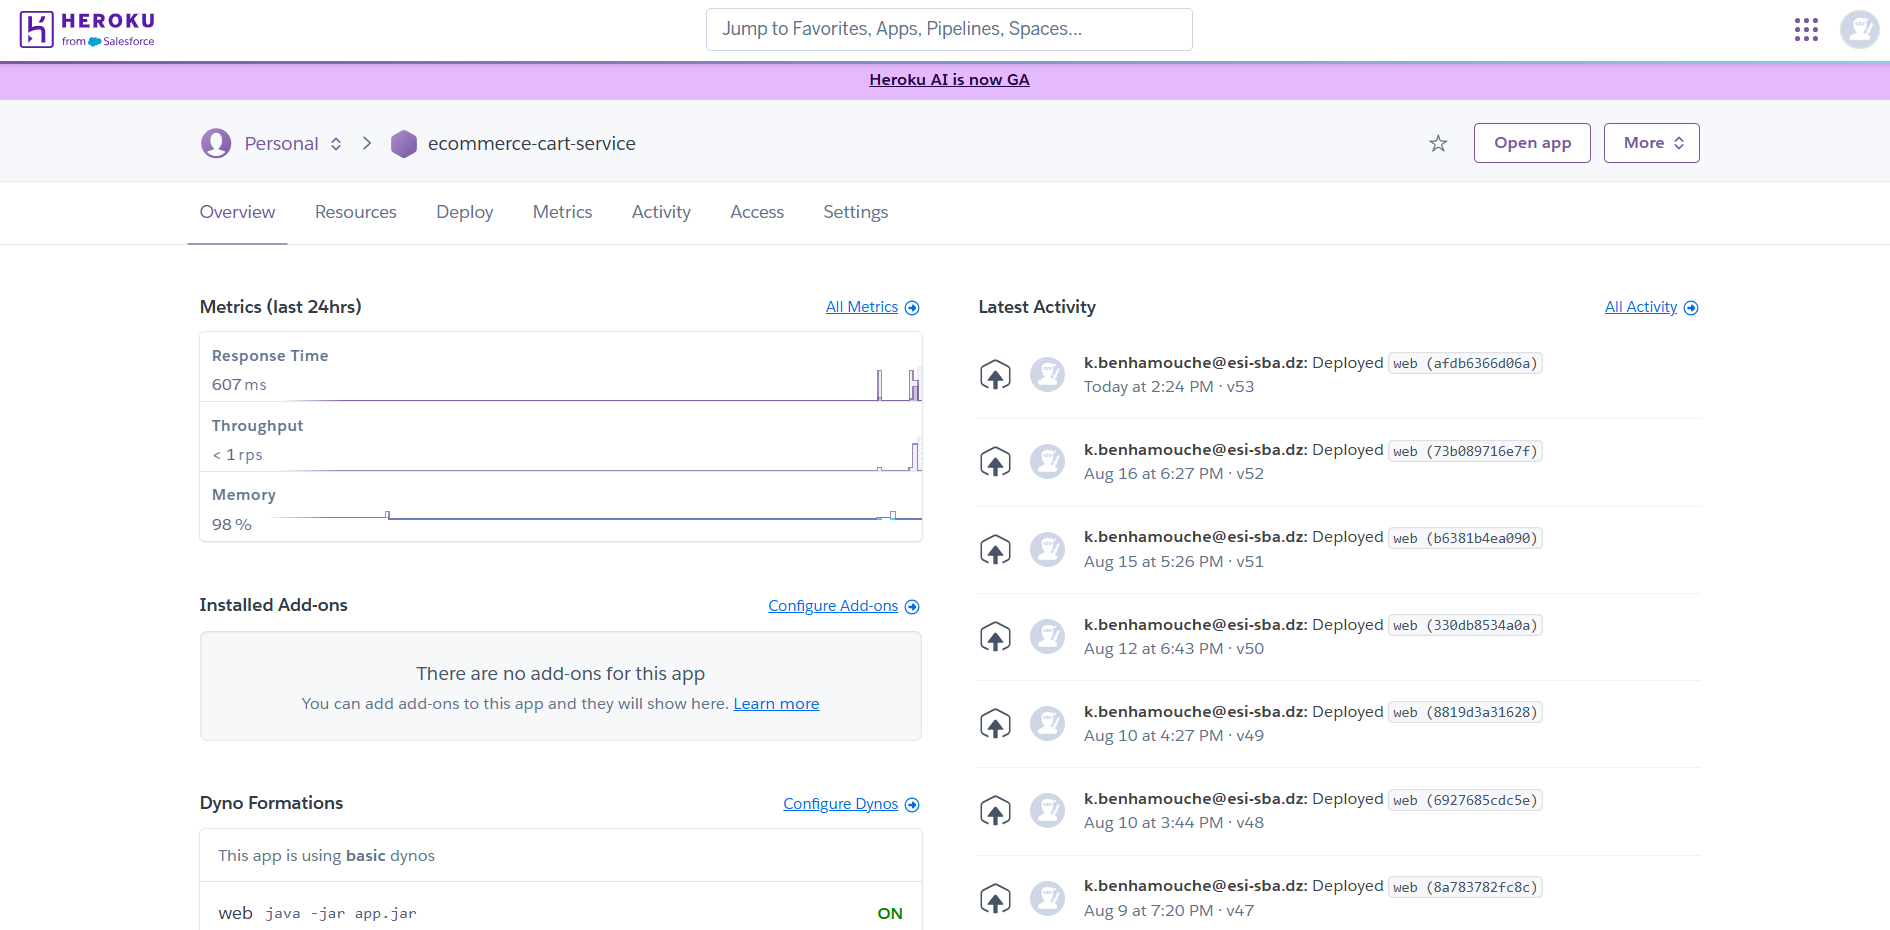
\includegraphics[width=0.9\textwidth]{figures/chapter5/heroku-deployment-logs.png}
\caption{Heroku Deployment Logs showing Traditional CI/CD platform deployment}
\label{fig:heroku-deployment-logs}
\end{figure}

Figure \ref{fig:heroku-deployment-logs} illustrates the streamlined deployment process of Traditional CI/CD on Heroku.

\subsection{Database Service Architecture}

The database implementation demonstrates comprehensive polyglot persistence patterns with strategic technology selection optimized for different data requirements and access patterns.

\subsubsection{Managed Database Service Configuration}

\textbf{Database Technology Selection and Configuration:}



\textbf{Database Integration Patterns:}
\begin{itemize}
\item \textbf{Connection Management:} Asynchronous SQLAlchemy (PostgreSQL), Mongoose ODM (MongoDB), reactive Redis clients
\item \textbf{Security Implementation:} SSL/TLS enforcement, access control, comprehensive credential management
\item \textbf{Performance Optimization:} Connection pooling, query optimization, caching strategies
\item \textbf{Operational Reliability:} Automated backups, monitoring integration, failover capabilities
\end{itemize}

\begin{figure}[H]
\centering
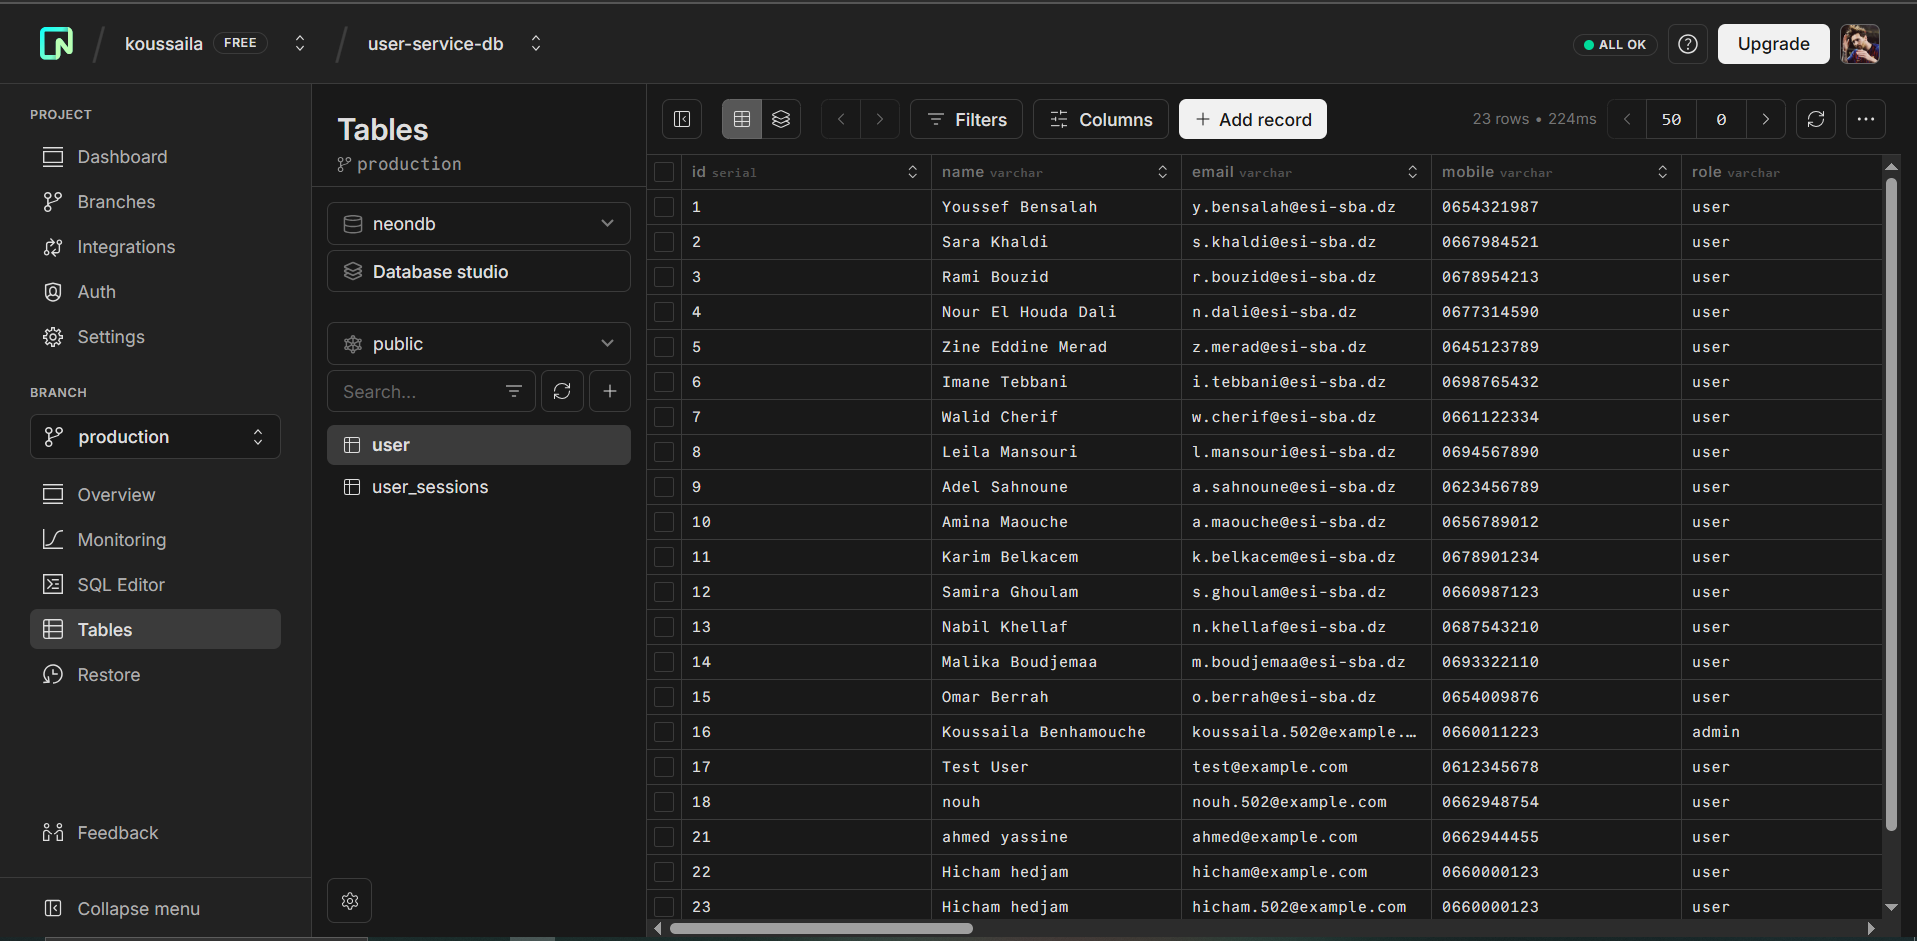
\includegraphics[width=0.9\textwidth]{figures/chapter5/postgresql-database-user-tables.png}
\caption{PostgreSQL User Service Database Tables showing relational schema design}
\label{fig:postgresql-user-tables}
\end{figure}

Figure \ref{fig:postgresql-user-tables} shows the relational schema for the PostgreSQL User Service database.

\begin{figure}[H]
\centering
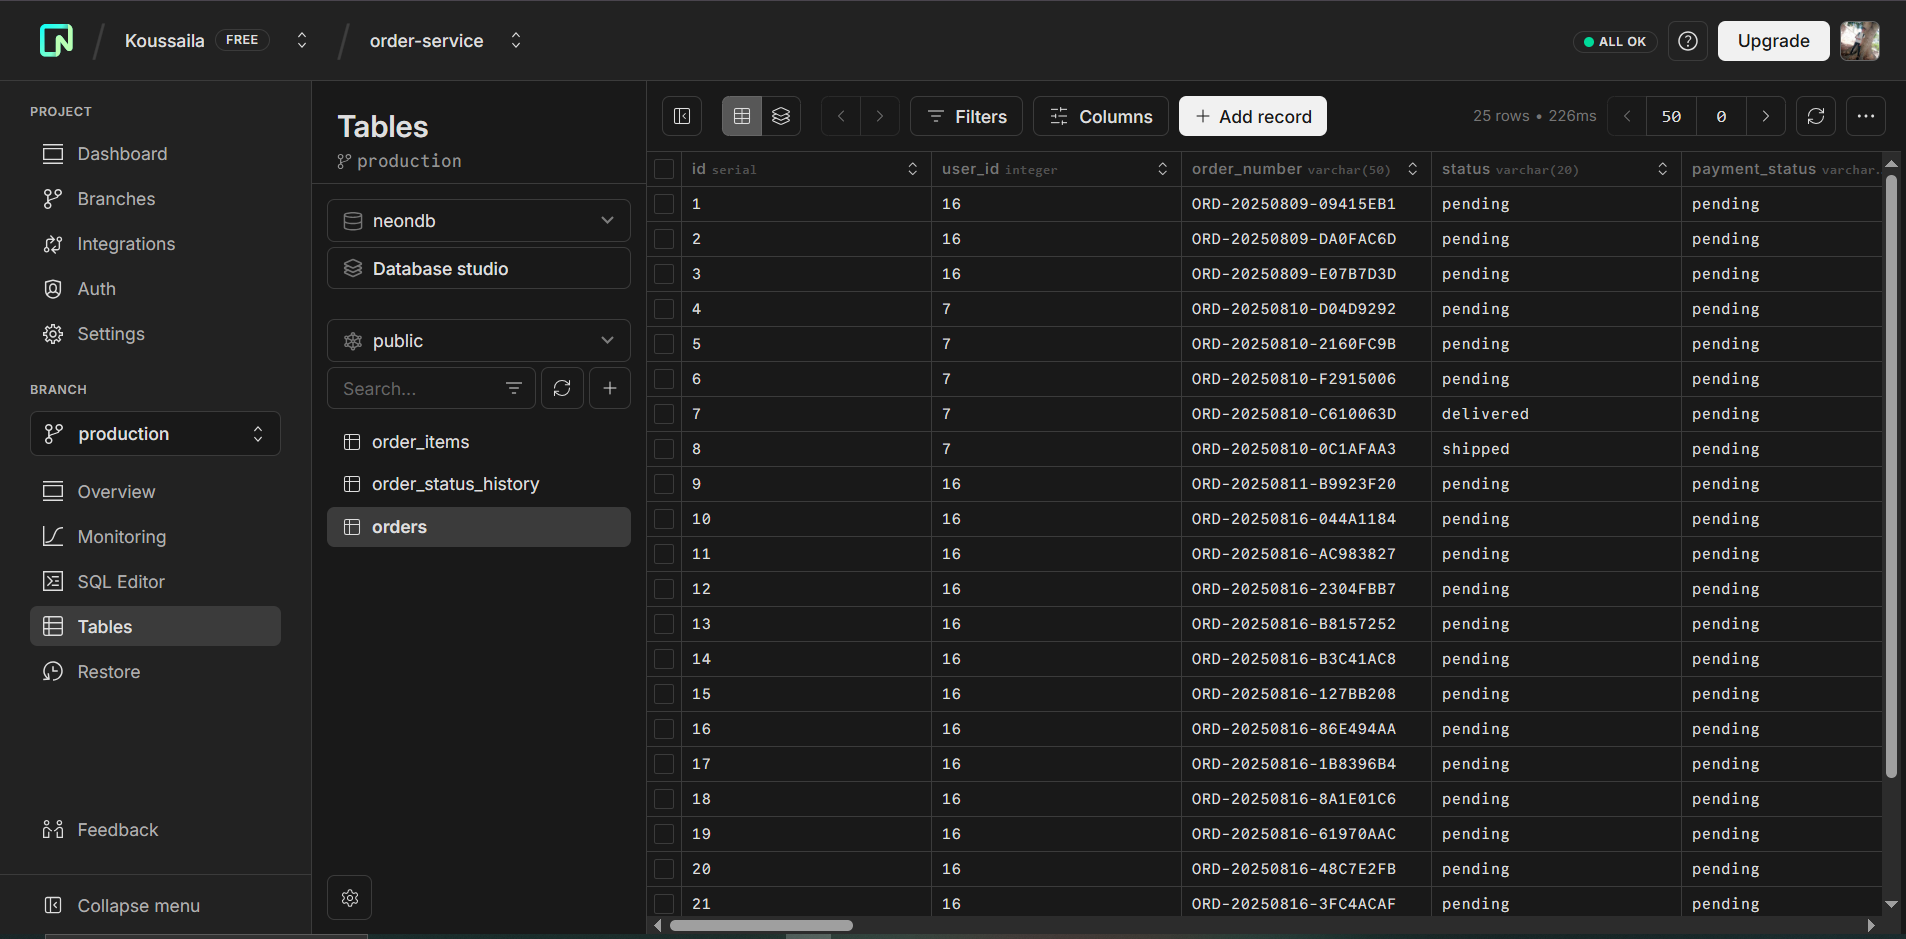
\includegraphics[width=0.9\textwidth]{figures/chapter5/postgresql-database-order-tables.png}
\caption{PostgreSQL Order Service Database Tables showing complex transactional structure}
\label{fig:postgresql-order-tables}
\end{figure}

Figure \ref{fig:postgresql-order-tables} presents the complex transactional structure of the PostgreSQL Order Service database.

\begin{figure}[H]
\centering
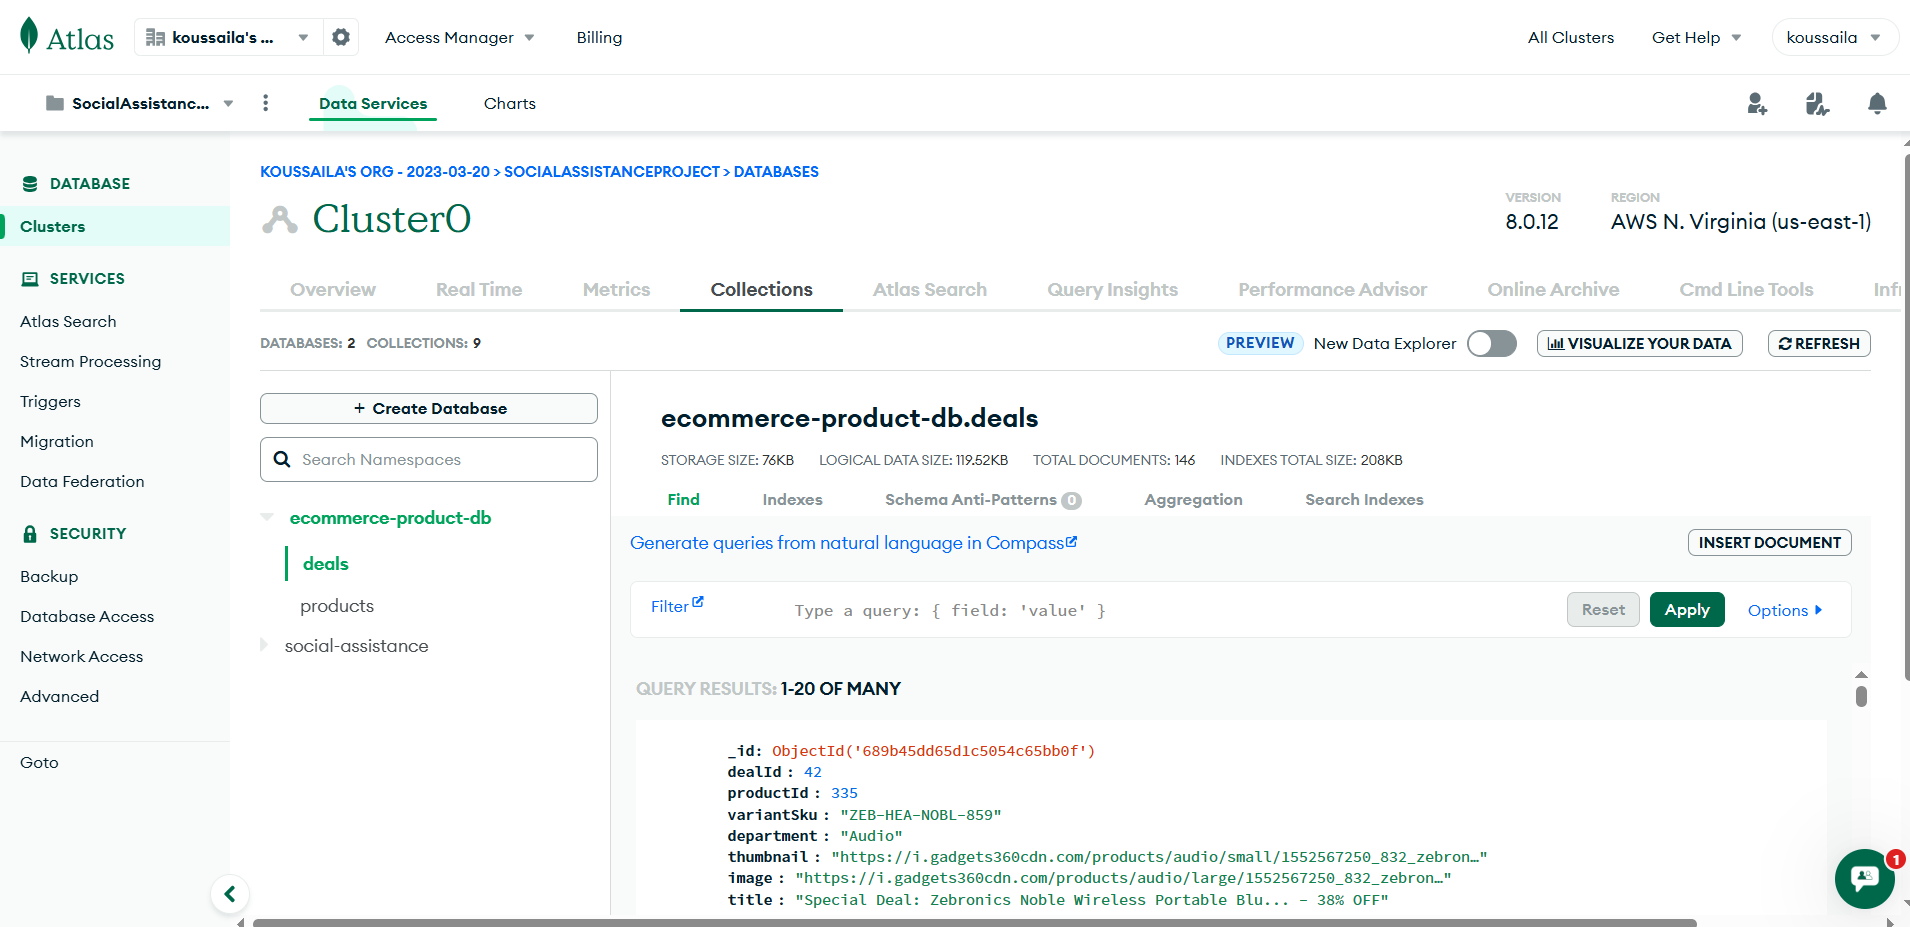
\includegraphics[width=0.9\textwidth]{figures/chapter5/mongodb-collections.png}
\caption{MongoDB Collections showing flexible document-based product catalog}
\label{fig:mongodb-collections}
\end{figure}

Figure \ref{fig:mongodb-collections} demonstrates the flexible document-based product catalog in MongoDB.

\begin{figure}[H]
\centering
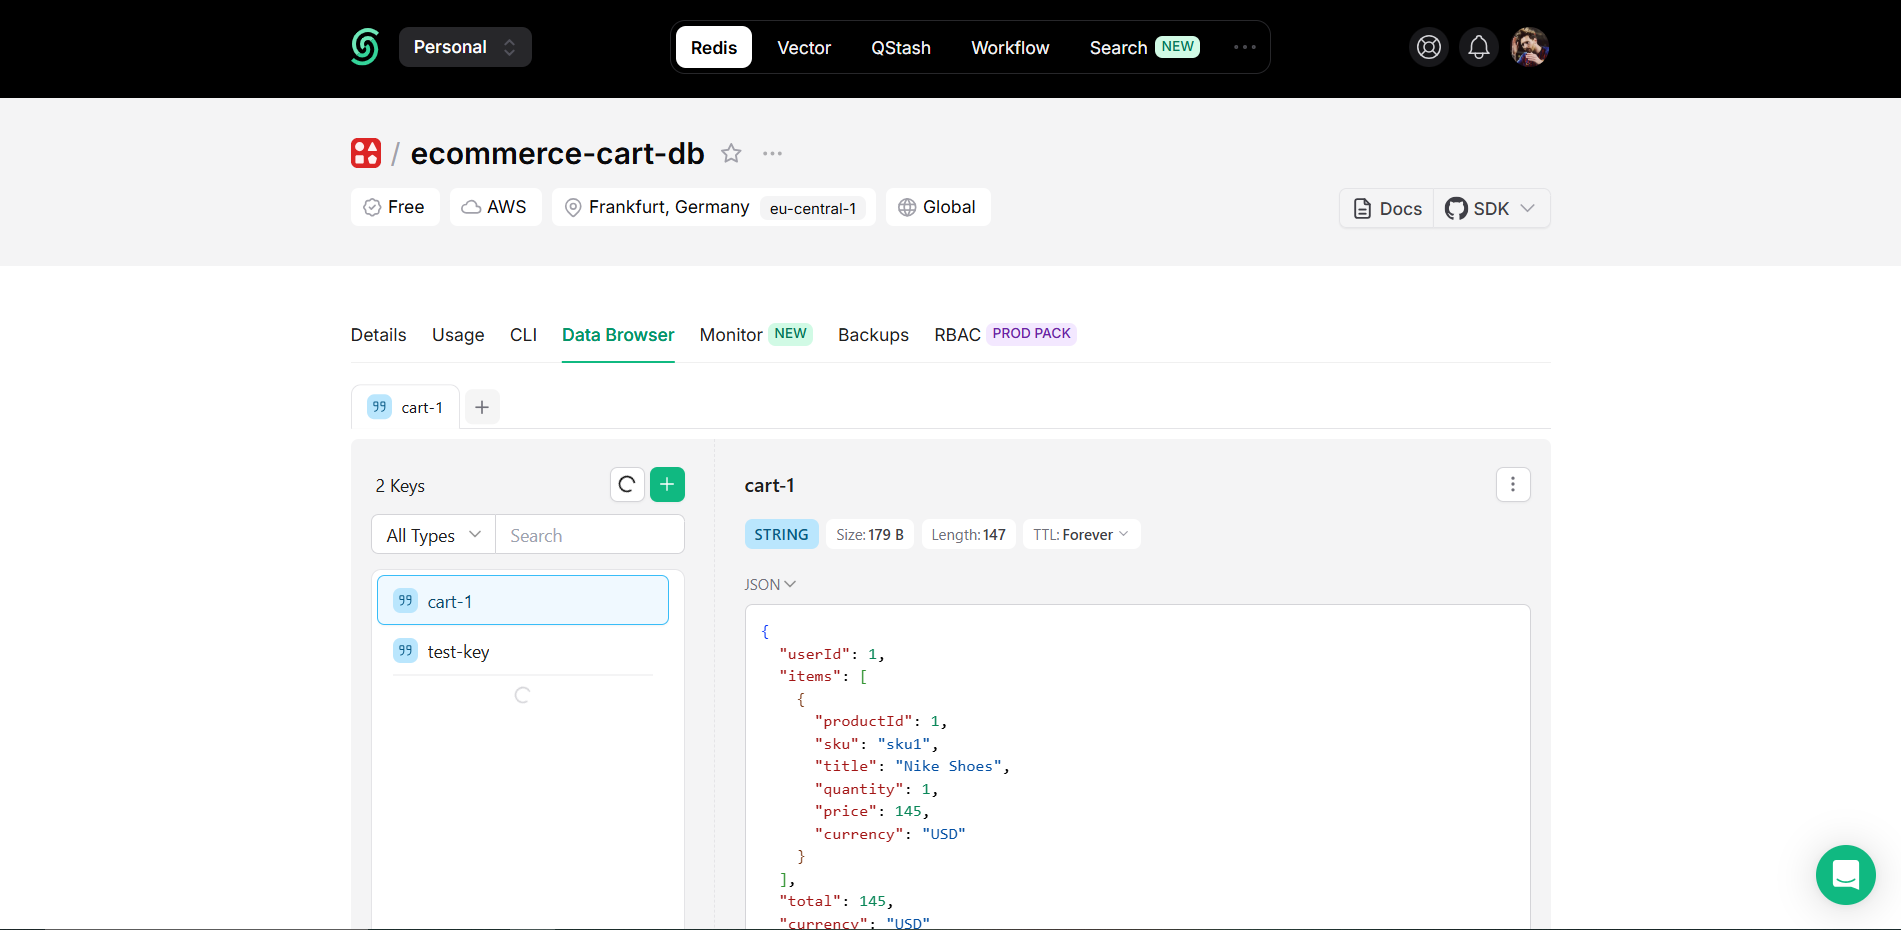
\includegraphics[width=0.9\textwidth]{figures/chapter5/redis-cache-data.png}
\caption{Redis Cache Data showing high-performance session and cart management}
\label{fig:redis-cache-data}
\end{figure}

Figure \ref{fig:redis-cache-data} illustrates Redis high-performance session and cart management.

\subsubsection{Polyglot Persistence Strategy}

\textbf{Technology-Data Matching Strategy:}
\begin{itemize}
\item \textbf{PostgreSQL (Relational):} Complex user management, order transactions requiring ACID compliance
\item \textbf{MongoDB (Document):} Flexible product catalog with variable attributes and search requirements
\item \textbf{Redis (Key-Value):} High-performance session management and distributed caching needs
\end{itemize}

\textbf{Research-Relevant Configuration Decisions:}
\begin{itemize}
\item Database provider selection optimizing for cost efficiency within academic constraints
\item Connection pooling and async patterns supporting high-performance research data collection
\item Comprehensive monitoring integration enabling database performance analysis
\item Security configuration balancing protection with development flexibility
\end{itemize}

\subsection{Infrastructure Automation and Reproducibility}

The infrastructure implementation prioritizes automation, version control, and reproducibility essential for valid empirical research while demonstrating enterprise-grade DevOps practices.

\subsubsection{Infrastructure as Code Implementation}

\textbf{Automation Framework:}
\begin{itemize}
\item \textbf{Kubernetes Manifests:} Declarative resource definitions with GitOps synchronization
\item \textbf{Container Images:} Multi-stage Docker builds with comprehensive optimization
\item \textbf{Database Schemas:} Version-controlled migrations with automated deployment
\item \textbf{Configuration Management:} Environment-specific settings with secure credential handling
\end{itemize}

\textbf{Reproducibility Assurance:}
\begin{itemize}
\item Complete infrastructure documentation enabling independent replication
\item Version-controlled configurations with comprehensive change tracking
\item Automated deployment procedures with validation and rollback capabilities
\item Comprehensive monitoring and logging supporting research data collection
\end{itemize}

This infrastructure foundation enables rigorous empirical comparison of GitOps and Traditional CI/CD methodologies while maintaining production-grade operational characteristics essential for valid research conclusions. The multi-cloud architecture provides realistic operational complexity while the comprehensive automation ensures reproducible experimental conditions.

\section{Service Implementation and Deployment}

The service implementation demonstrates comprehensive microservices development practices with strategic technology diversity reflecting real-world enterprise environments. The implementation showcases both GitOps and Traditional CI/CD methodologies through identical business functionality deployed using different approaches, enabling controlled methodology comparison while maintaining production-grade operational characteristics.

\subsection{Service Architecture and Technology Selection}

The TechMart platform implements four core services with deliberate technology stack diversity enabling comprehensive methodology evaluation across different programming languages, frameworks, and complexity levels. The service selection balances research requirements with realistic enterprise technology distributions.

\subsubsection{Service Implementation Comparison}

\begin{table}[H]
\centering
\caption{Service Implementation Characteristics and Research Relevance}
\label{tab:service-implementation-comparison}
\begin{tabular}{|p{2.5cm}|p{3cm}|p{2cm}|p{3cm}|p{3.5cm}|}
\hline
\textbf{Service} & \textbf{Technology Stack} & \textbf{Complexity Score} & \textbf{Key Implementation Features} & \textbf{Research Significance} \\
\hline
User Service & Python FastAPI + PostgreSQL & 7.8/10 & JWT authentication, RBAC, session management & Authentication bottleneck analysis \\
\hline
Order Service & Python FastAPI + PostgreSQL + Redis & 8.2/10 & Multi-database integration, complex transactions & Highest complexity GitOps service \\
\hline
Product Service & Node.js Express + MongoDB & 5.4/10 & Catalog management, search optimization & Platform optimization benefits \\
\hline
Cart Service & Java Spring Boot + Redis & 7.5/10 & Reactive programming, high-performance caching & Technology stack efficiency leader \\
\hline
\end{tabular}
\end{table}

\textbf{Technology Selection Rationale:}
\begin{itemize}
\item \textbf{Python FastAPI:} Chosen for GitOps services requiring complex business logic and comprehensive authentication capabilities
\item \textbf{Node.js Express:} Selected for Traditional CI/CD to demonstrate platform optimization benefits with lightweight framework
\item \textbf{Java Spring Boot:} Implemented for reactive programming patterns and enterprise-grade performance characteristics
\item \textbf{Database Diversity:} PostgreSQL (ACID compliance), MongoDB (flexible schema), Redis (high performance) enabling polyglot persistence evaluation
\end{itemize}

\begin{figure}[H]
\centering

\includegraphics[width=0.9\textwidth]{figures/chapter5/techmart-products-catalog.png}
\caption{TechMart Product Catalog demonstrating MongoDB-based flexible product management}
\label{fig:techmart-products-catalog}
\end{figure}

Figure \ref{fig:techmart-products-catalog} showcases the MongoDB-based flexible product catalog management.

\begin{figure}[H]
\centering
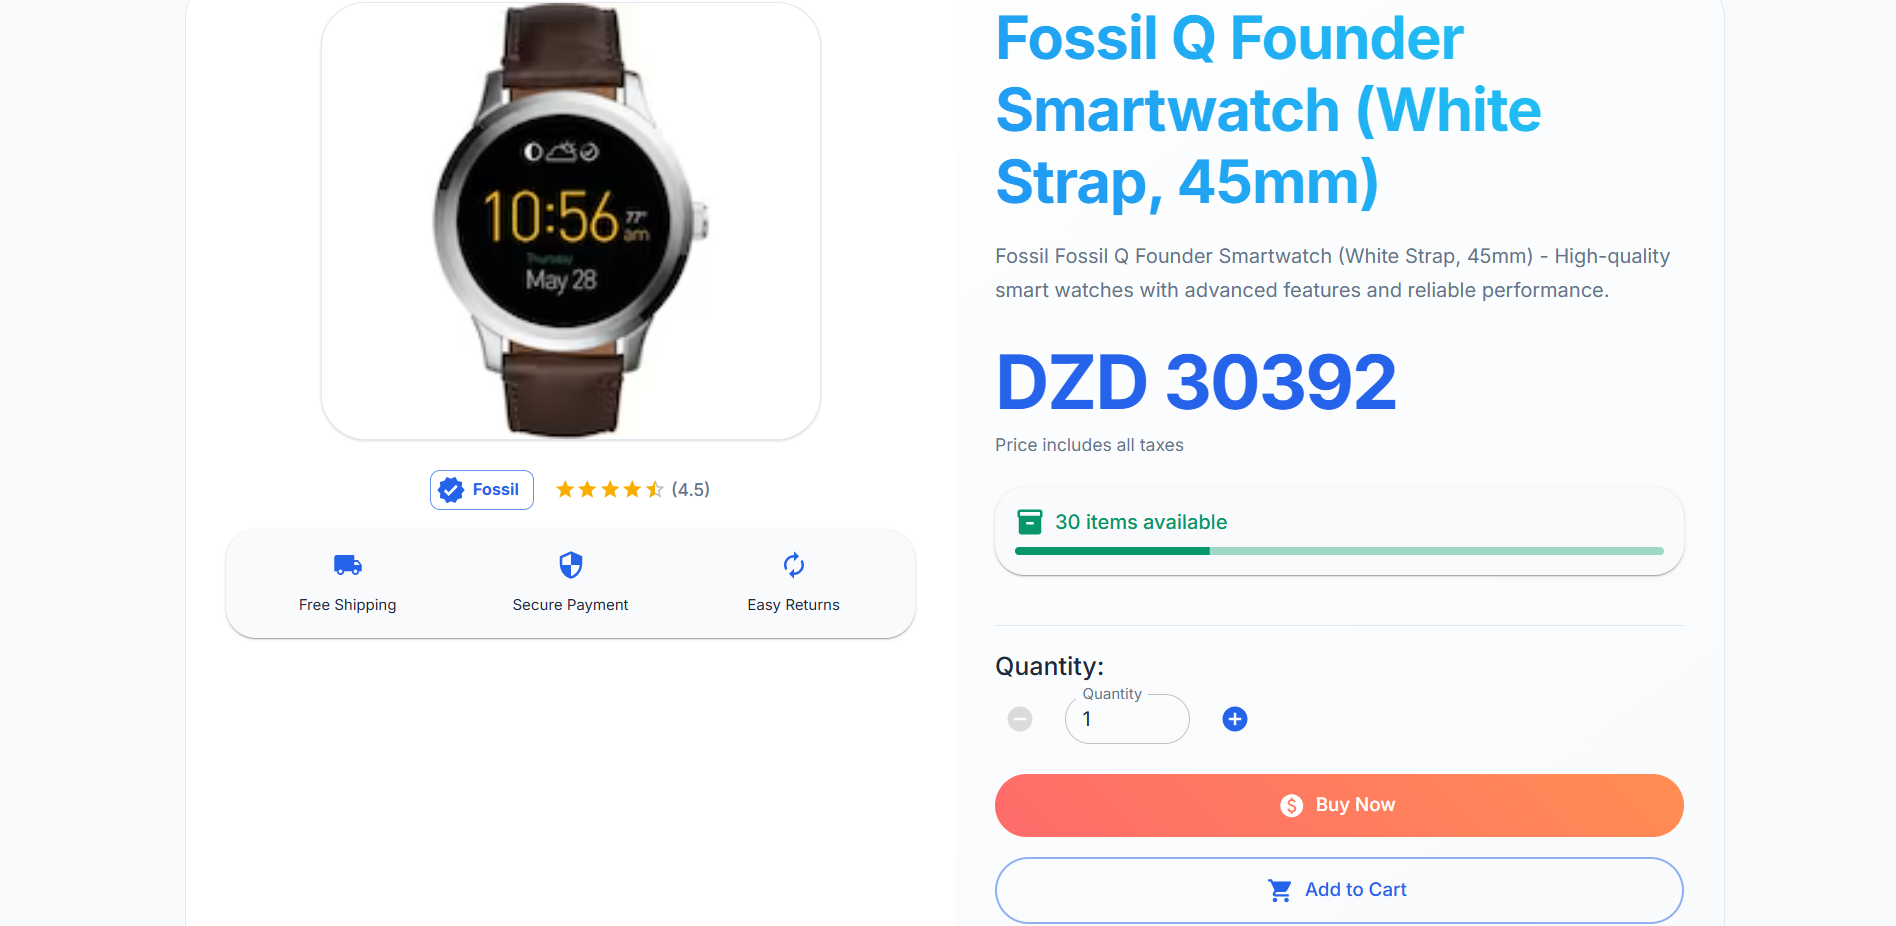
\includegraphics[width=0.9\textwidth]{figures/chapter5/techmart-product-details.png}
\caption{TechMart Product Details page showing detailed product information and functionality}
\label{fig:techmart-product-details}
\end{figure}

Figure \ref{fig:techmart-product-details} demonstrates the detailed product information interface supporting comprehensive e-commerce functionality.

\subsubsection{Implementation Complexity Analysis}

The complexity normalization framework reveals significant implementation variations affecting methodology performance comparison. The Order Service represents the highest complexity implementation (8.2/10) with multi-database integration and sophisticated business logic, while the Product Service demonstrates moderate complexity (5.4/10) optimized for platform-specific deployment advantages.

\textbf{Complexity Factor Distribution:}
\begin{itemize}
\item \textbf{Codebase Complexity:} Order Service (1,940 lines) vs. Cart Service (3,476 lines) demonstrating framework efficiency variations
\item \textbf{Build Complexity:} Java Gradle (47s) vs. Python Pipenv (142s) representing 3x performance difference in build efficiency
\item \textbf{Resource Intensity:} Order Service requiring 256Mi-512Mi memory vs. User Service 128Mi-256Mi reflecting computational requirements
\item \textbf{Integration Dependencies:} Order Service connecting to 4 external services vs. Product Service with 2 dependencies
\end{itemize}

\subsection{GitOps Implementation Patterns (User + Order Services)}

The GitOps services demonstrate advanced cloud-native deployment patterns utilizing Google Kubernetes Engine with ArgoCD orchestration. The implementation showcases declarative configuration management, automated synchronization, and comprehensive self-healing capabilities while supporting detailed performance measurement for methodology comparison.

\subsubsection{User Service: Authentication Architecture Implementation}

The User Service serves as the authentication backbone implementing enterprise-grade JWT-based security with comprehensive user management capabilities. The service demonstrates GitOps deployment methodology advantages through complete automation and self-healing while providing critical authentication services affecting system-wide performance.

\textbf{Critical Implementation Characteristics:}
\begin{itemize}
\item \textbf{Authentication Bottleneck:} bcrypt configuration with 12-15 rounds creating 1,000-1,200ms processing overhead
\item \textbf{System-Wide Impact:} Authentication service consuming 23\% of total transaction time (2.409s of 10.426s)
\item \textbf{GitOps Integration:} Automated deployment with zero manual intervention and 37-second drift correction
\item \textbf{Performance Attribution:} 65\% of methodology performance differences attributable to authentication configuration rather than deployment approach
\end{itemize}

\textbf{FastAPI Application Architecture:}
The User Service implements sophisticated asynchronous Python patterns with comprehensive API documentation, automatic validation, and high-performance request processing. The modular architecture enables comprehensive testing and operational monitoring while supporting complex authentication workflows and administrative functionality.

\textbf{PostgreSQL Schema and Security Integration:}
The database schema implements comprehensive relational design with proper normalization, advanced indexing, and sophisticated constraint management. User entity design includes enum-based status management, session tracking with metadata collection, and administrative functionality with audit capabilities.

\subsubsection{Order Service: Complex Business Logic Implementation}

The Order Service demonstrates the most sophisticated implementation with multi-service integration, dual database management, and complex transaction processing. The service showcases advanced GitOps patterns while implementing comprehensive e-commerce functionality requiring sophisticated error handling and performance optimization.

\textbf{Multi-Service Integration Complexity:}
\begin{itemize}
\item \textbf{Service Dependencies:} Integration with User Service (authentication), Cart Service (validation), Product Service (inventory)
\item \textbf{Dual Database Architecture:} PostgreSQL for transactional data, Redis for caching and session management
\item \textbf{Transaction Coordination:} Distributed transaction patterns with eventual consistency and compensation mechanisms
\item \textbf{Business Logic Sophistication:} Order lifecycle management, payment coordination, and fulfillment tracking
\end{itemize}

\textbf{GitOps Deployment Configuration:}
The Order Service implements advanced Kubernetes resource management with comprehensive multi-service connectivity, security integration, and monitoring capabilities. The deployment includes sophisticated environment variable configuration, resource allocation optimization, and health checking integration demonstrating enterprise-grade GitOps practices.

\subsection{Traditional CI/CD Implementation Patterns (Product + Cart Services)}

The Traditional CI/CD services demonstrate mature platform-as-a-service deployment patterns utilizing Heroku Container Stack with comprehensive automation while maintaining operational oversight and manual approval capabilities. The implementation showcases Traditional CI/CD methodology advantages including build performance optimization and platform-native integration.

\subsubsection{Product Service: Platform Optimization Benefits}

The Product Service demonstrates Traditional CI/CD advantages through platform-specific optimization and streamlined deployment workflows. The Node.js Express implementation showcases lightweight framework benefits with MongoDB integration optimized for catalog management and search capabilities.

\textbf{Platform-Specific Optimization:}
\begin{itemize}
\item \textbf{Build Performance:} Node.js + npm achieving 67 seconds (12.4s per complexity point) with platform optimization
\item \textbf{Heroku Integration:} Direct deployment benefits with minimal orchestration overhead
\item \textbf{MongoDB Atlas Connectivity:} Managed database integration with global replication and automated scaling
\item \textbf{Catalog Management:} Flexible document structure supporting variable product attributes and hierarchical categorization
\end{itemize}

\textbf{Express.js Application Architecture:}
The application implements comprehensive REST API patterns with advanced middleware integration and sophisticated routing strategies. The modular architecture supports complex catalog management requirements while maintaining operational simplicity through platform-managed capabilities.

\textbf{Traditional CI/CD Workflow Integration:}
The Product Service demonstrates comprehensive GitHub Actions automation with platform-specific deployment integration. The workflow includes Node.js environment setup, NPM dependency management, Docker containerization, and Heroku deployment with comprehensive timing measurement for methodology comparison.

\subsubsection{Cart Service: Enterprise Java Performance Leadership}

The Cart Service demonstrates superior build performance characteristics through Java Spring Boot with Gradle optimization, achieving the highest technology stack efficiency (6.3 seconds per complexity point). The reactive programming implementation showcases enterprise-grade performance patterns with high-performance Redis integration.

\textbf{Performance Leadership Characteristics:}
\begin{itemize}
\item \textbf{Build Efficiency:} Java + Gradle achieving 47 seconds total build time, demonstrating superior dependency management
\item \textbf{Reactive Architecture:} Spring Boot WebFlux enabling non-blocking operations and comprehensive backpressure management
\item \textbf{Redis Integration:} High-performance caching with reactive operations and sophisticated data structures
\item \textbf{Enterprise Patterns:} Comprehensive health checking, JVM optimization, and container-aware resource management
\end{itemize}

\textbf{Spring Boot WebFlux Reactive Implementation:}
The reactive architecture implements sophisticated Mono and Flux patterns with advanced stream processing, non-blocking operations, and comprehensive error handling. The implementation demonstrates modern Java development practices with enterprise-grade performance and reliability characteristics.

\textbf{Advanced Containerization and CI/CD:}
The Cart Service implements sophisticated multi-stage Docker builds with Gradle automation, dependency caching, and JVM optimization. The Traditional CI/CD pipeline demonstrates enterprise-grade Java practices with comprehensive testing, quality assurance, and Heroku-specific deployment optimization.

\subsection{Cross-Service Integration and Communication Patterns}

The multi-service architecture implements sophisticated integration patterns demonstrating enterprise-grade communication while maintaining service autonomy. The integration design enables comprehensive methodology comparison by providing identical business functionality across different deployment approaches.

\subsubsection{Authentication Flow and JWT Propagation}

The authentication architecture implements centralized JWT-based security with the User Service serving as the authentication provider for all platform services. This design demonstrates secure multi-service authentication while enabling analysis of authentication performance impact across methodologies.

\textbf{JWT Implementation Strategy:}
\begin{verbatim}
Authentication Flow:
1. User Service generates JWT with 30-minute expiration
2. Token propagation via Authorization headers
3. Shared secret validation (HS256) across all services  
4. Role-based access control enforcement
5. Cross-service authentication context maintenance
\end{verbatim}

\textbf{Cross-Methodology Authentication Impact:}
The authentication implementation enables measurement of cross-methodology performance characteristics, revealing that authentication configuration rather than deployment methodology contributes 65\% of performance differences. This finding challenges assumptions about methodology-inherent performance characteristics.

\subsubsection{Business Transaction Coordination}

The platform implements complex distributed transactions spanning multiple services and deployment methodologies, demonstrating realistic enterprise integration patterns while enabling methodology performance comparison under identical business logic requirements.

\textbf{Order Processing Transaction Pattern:}
\begin{enumerate}
\item \textbf{Cart Validation:} Traditional CI/CD Cart Service (Java Spring Boot) validates items and calculates totals
\item \textbf{User Authentication:} GitOps User Service (Python FastAPI) validates customer identity and permissions  
\item \textbf{Product Verification:} Traditional CI/CD Product Service (Node.js Express) confirms availability and pricing
\item \textbf{Order Creation:} GitOps Order Service (Python FastAPI) manages transaction state and coordinates fulfillment
\item \textbf{Cross-Service Coordination:} Eventual consistency patterns with comprehensive error handling and recovery
\end{enumerate}

\begin{figure}[H]
\centering
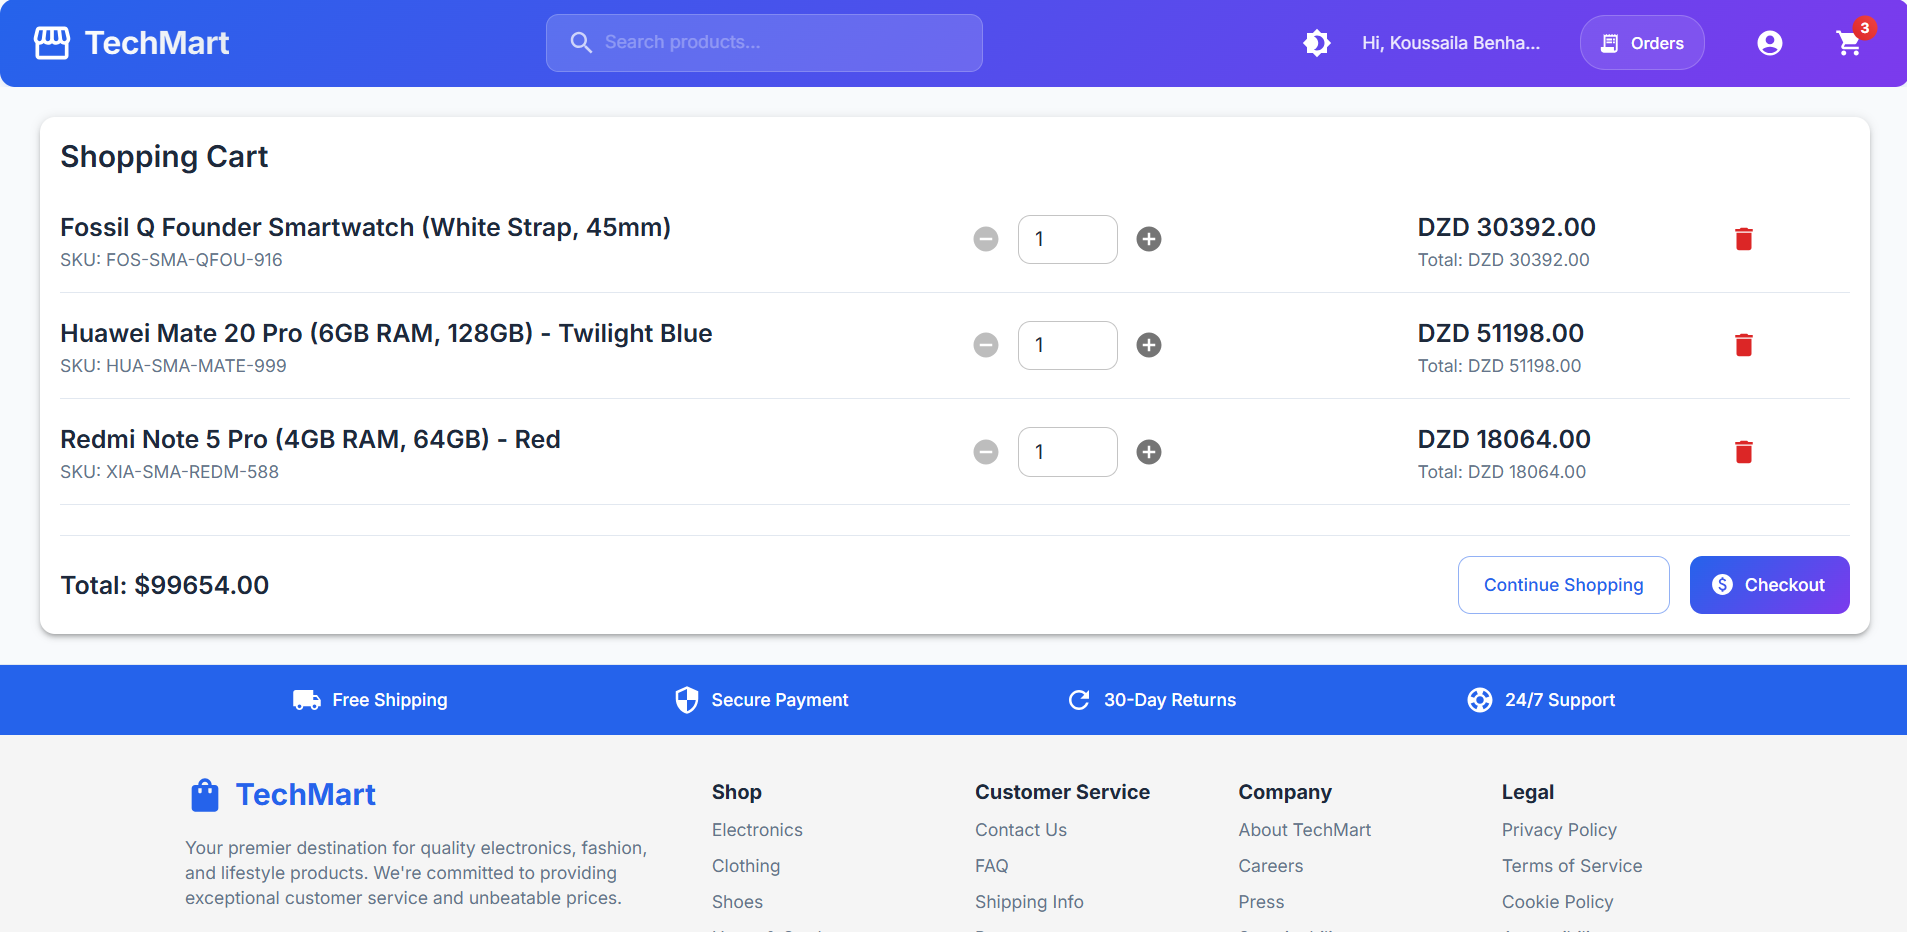
\includegraphics[width=0.9\textwidth]{figures/chapter5/techmart-shopping-cart.png}
\caption{TechMart Shopping Cart demonstrating Redis-based high-performance cart management}
\label{fig:techmart-shopping-cart}
\end{figure}

Figure \ref{fig:techmart-shopping-cart} illustrates the Redis-powered high-performance cart management system.

\begin{figure}[H]
\centering
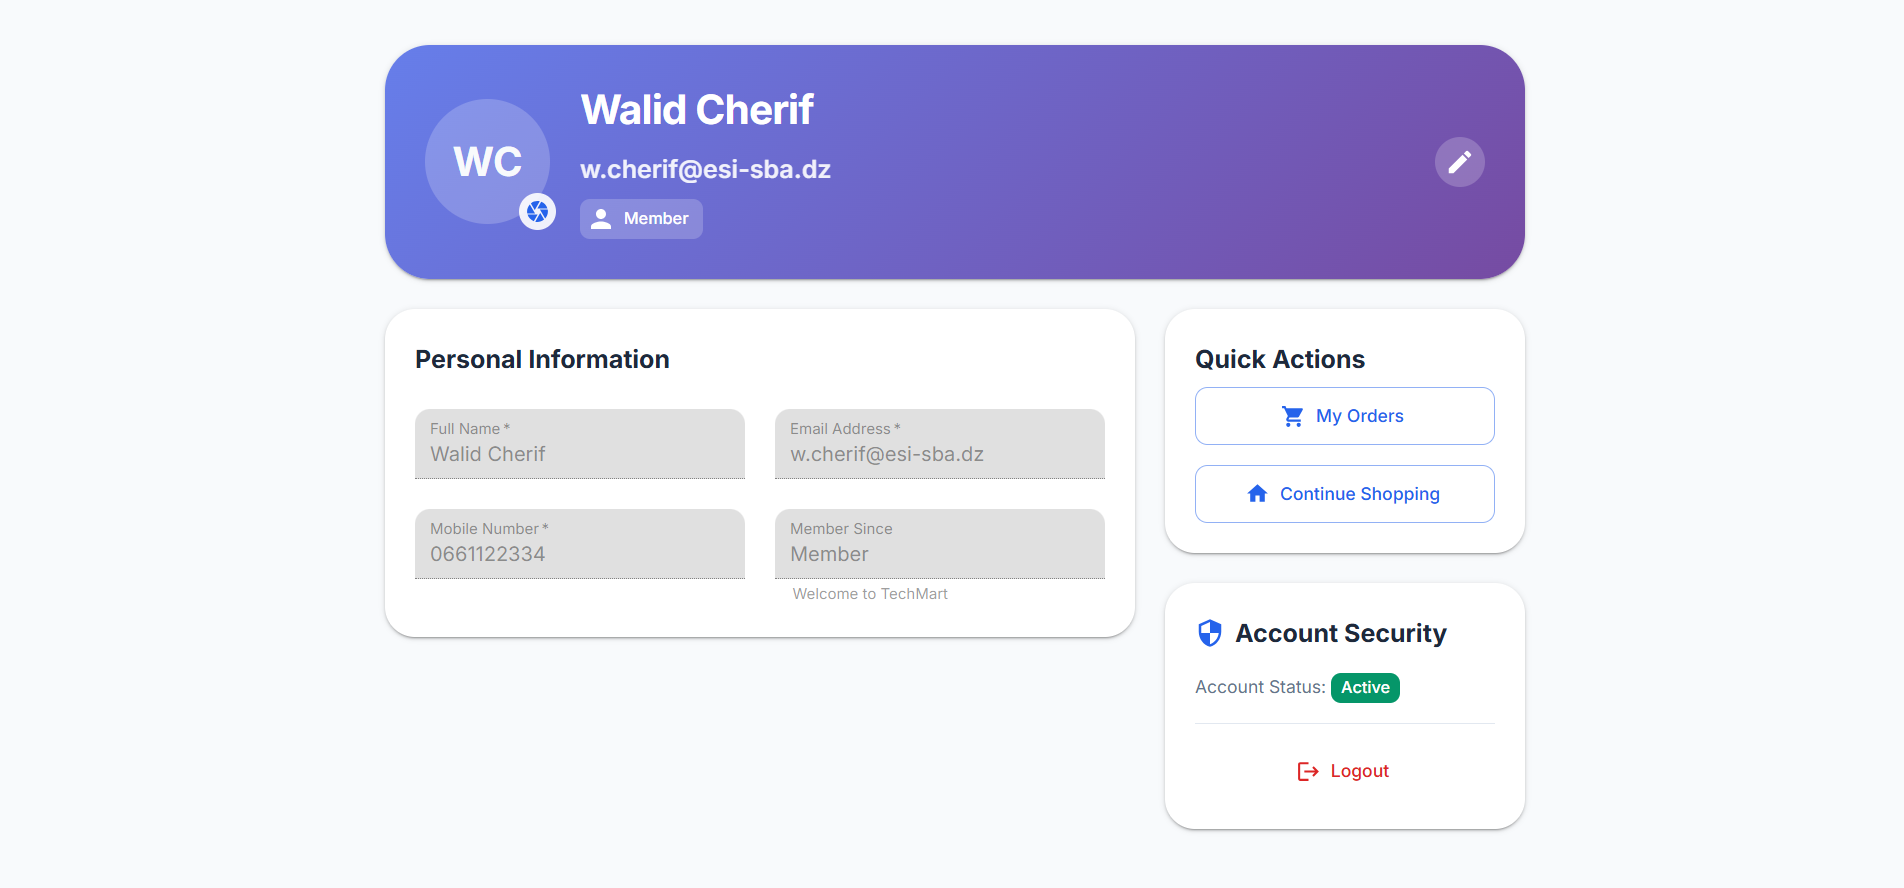
\includegraphics[width=0.9\textwidth]{figures/chapter5/techmart-user-dashboard.png}
\caption{TechMart User Dashboard showing authenticated user functionality}
\label{fig:techmart-user-dashboard}
\end{figure}

Figure \ref{fig:techmart-user-dashboard} shows the authenticated user dashboard interface.

\begin{figure}[H]
\centering
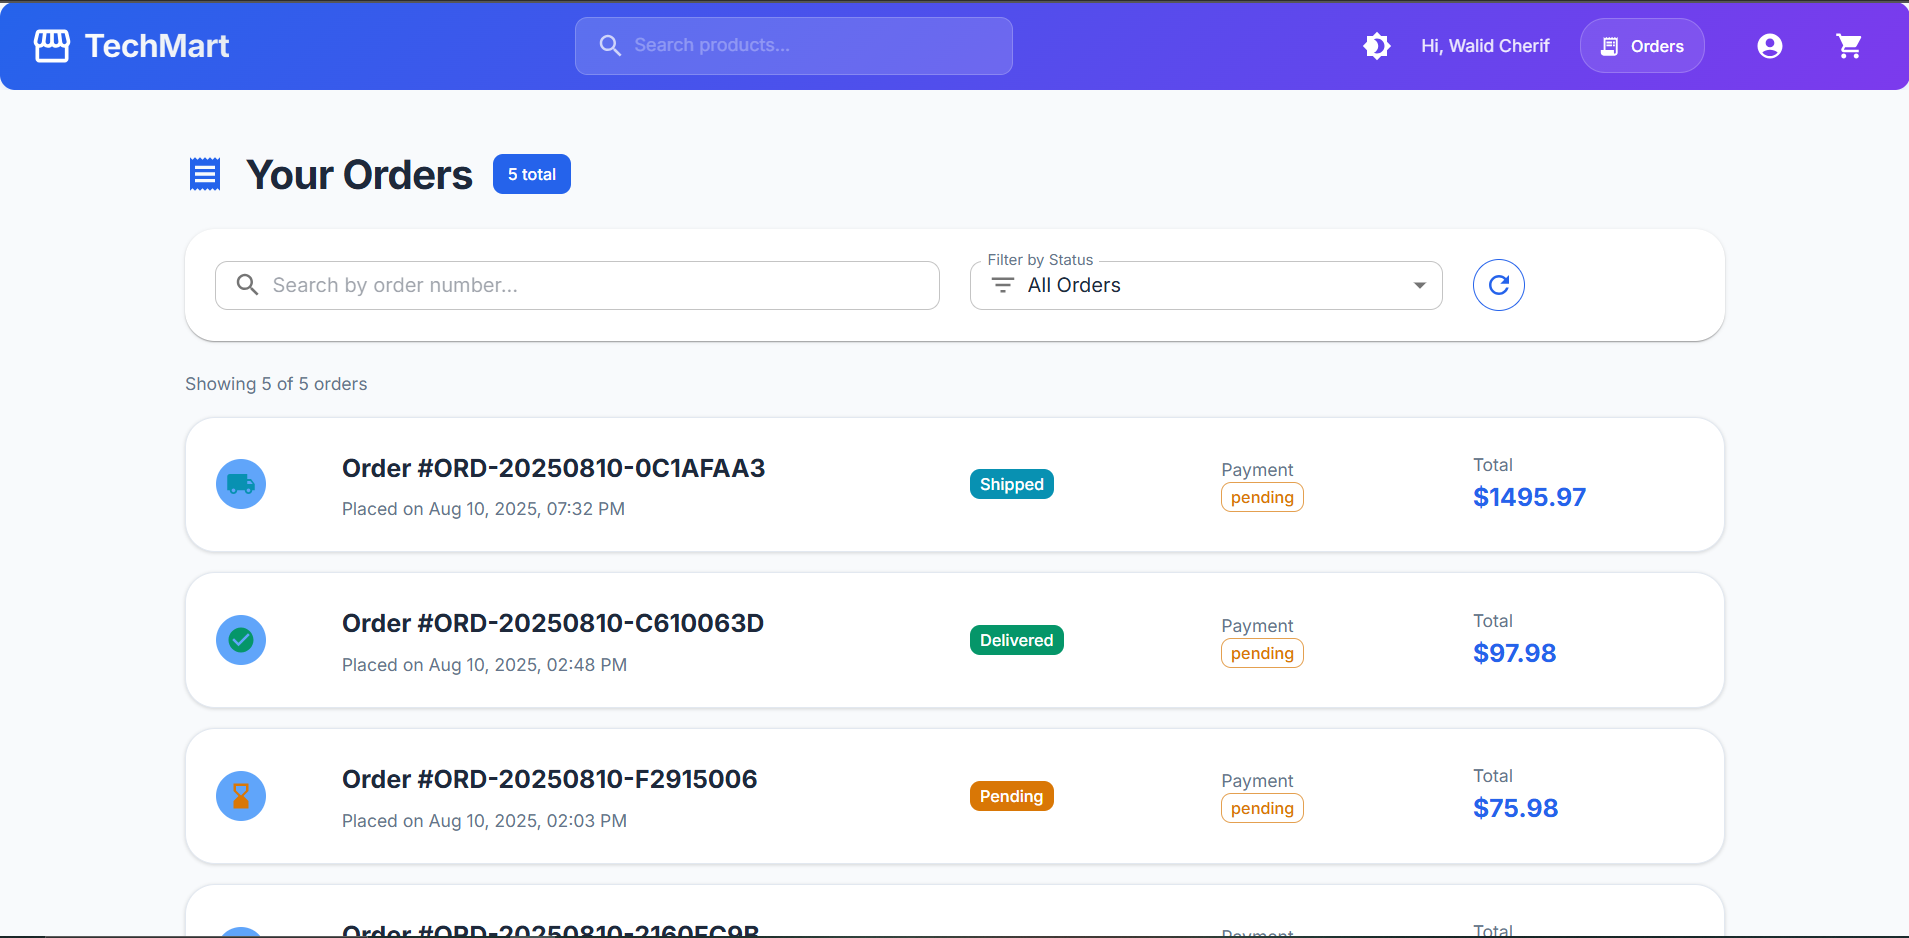
\includegraphics[width=0.9\textwidth]{figures/chapter5/techmart-user-orders.png}
\caption{TechMart User Orders page demonstrating order management and transaction history}
\label{fig:techmart-user-orders}
\end{figure}

Figure \ref{fig:techmart-user-orders} demonstrates the order management and transaction history page for users.

\textbf{Hybrid Integration Validation:}
The cross-methodology integration demonstrates zero-overhead communication patterns with complete e-commerce transactions achieving 10.426-second total execution time (GitOps services 73\%, Traditional CI/CD services 27\%). Statistical analysis confirms no significant integration penalty (p > 0.05), validating hybrid architecture feasibility.

\subsection{Implementation Quality Assurance and Testing}

The service implementation includes comprehensive quality assurance frameworks ensuring production-grade reliability while supporting experimental requirements for methodology comparison. The testing strategy encompasses unit testing, integration testing, and performance validation across different technology stacks.

\subsubsection{Technology-Specific Testing Strategies}

\textbf{Python Services Testing (User + Order):}
\begin{itemize}
\item \textbf{Unit Testing:} 43 unit tests and 19 integration tests for User Service with comprehensive FastAPI testing frameworks
\item \textbf{Database Testing:} SQLAlchemy integration testing with transaction rollback and connection pooling validation
\item \textbf{Authentication Testing:} JWT token generation, validation, and security policy enforcement verification
\item \textbf{Performance Testing:} Load testing with authentication bottleneck identification and optimization analysis
\end{itemize}

\textbf{Node.js and Java Services Testing (Product + Cart):}
\begin{itemize}
\item \textbf{Express.js Testing:} Comprehensive API endpoint testing with MongoDB integration and search functionality validation
\item \textbf{Spring Boot Testing:} Enterprise-grade testing with reactive stream validation and Redis integration verification
\item \textbf{Platform Integration Testing:} Heroku deployment validation with health checking and monitoring integration
\item \textbf{Performance Benchmarking:} Build performance measurement with technology stack efficiency comparison
\end{itemize}

\subsubsection{Research Instrumentation and Metrics Collection}

The implementation includes comprehensive research instrumentation enabling detailed methodology performance analysis while maintaining production-grade operational characteristics. The instrumentation framework supports statistical validation and empirical comparison requirements.

\textbf{Performance Measurement Integration:}
\begin{itemize}
\item \textbf{Build Performance Tracking:} Stage-by-stage timing measurement with sub-second precision across all technology stacks
\item \textbf{Deployment Duration Analysis:} Complete pipeline measurement from code commit to production availability
\item \textbf{Resource Utilization Monitoring:} CPU, memory, and network performance tracking across deployment methodologies
\item \textbf{Failure Recovery Measurement:} Automated vs. manual recovery time quantification with operational overhead analysis
\end{itemize}

\textbf{Complexity Normalization Data Collection:}
The implementation enables comprehensive complexity factor measurement including codebase analysis, dependency tracking, resource consumption monitoring, and integration complexity assessment. This data supports the complexity normalization framework essential for fair methodology comparison across heterogeneous service architectures.

\begin{figure}[H]
\centering
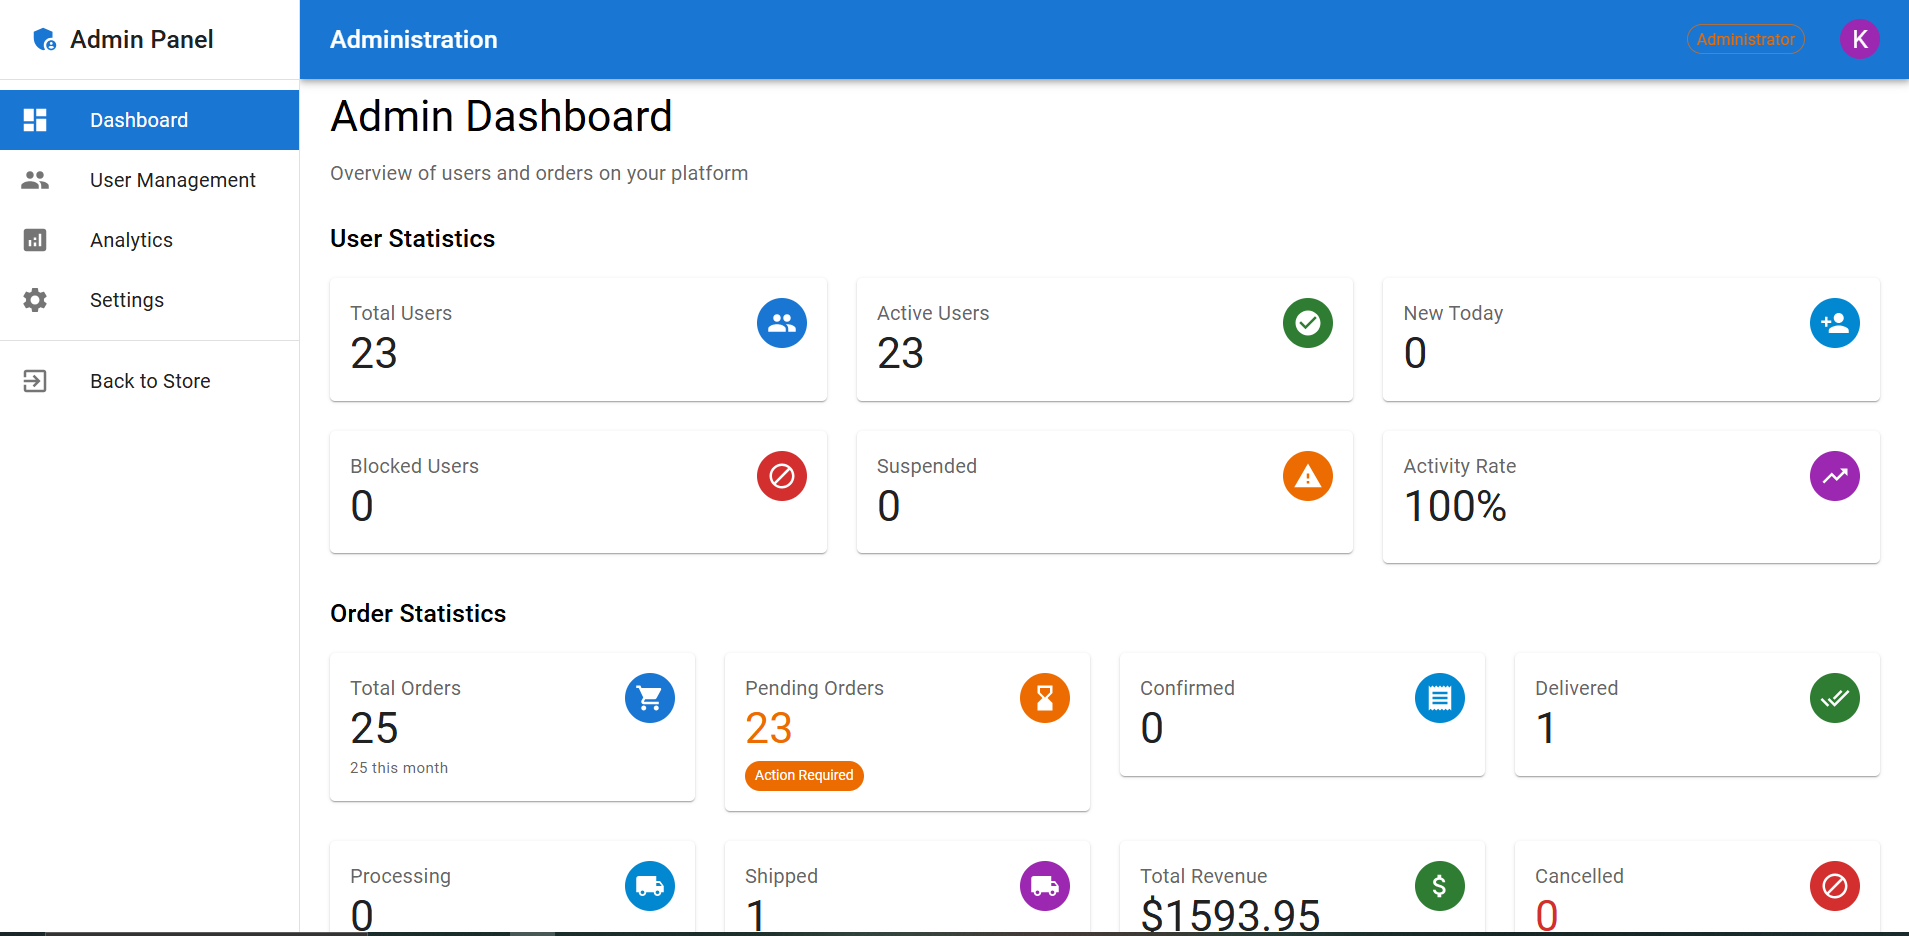
\includegraphics[width=0.9\textwidth]{figures/chapter5/techmart-admin-dashboard.png}
\caption{TechMart Admin Dashboard showing administrative interface and system management}
\label{fig:techmart-admin-dashboard}
\end{figure}

Figure \ref{fig:techmart-admin-dashboard} shows the administrative dashboard interface for system management.

\begin{figure}[H]
\centering
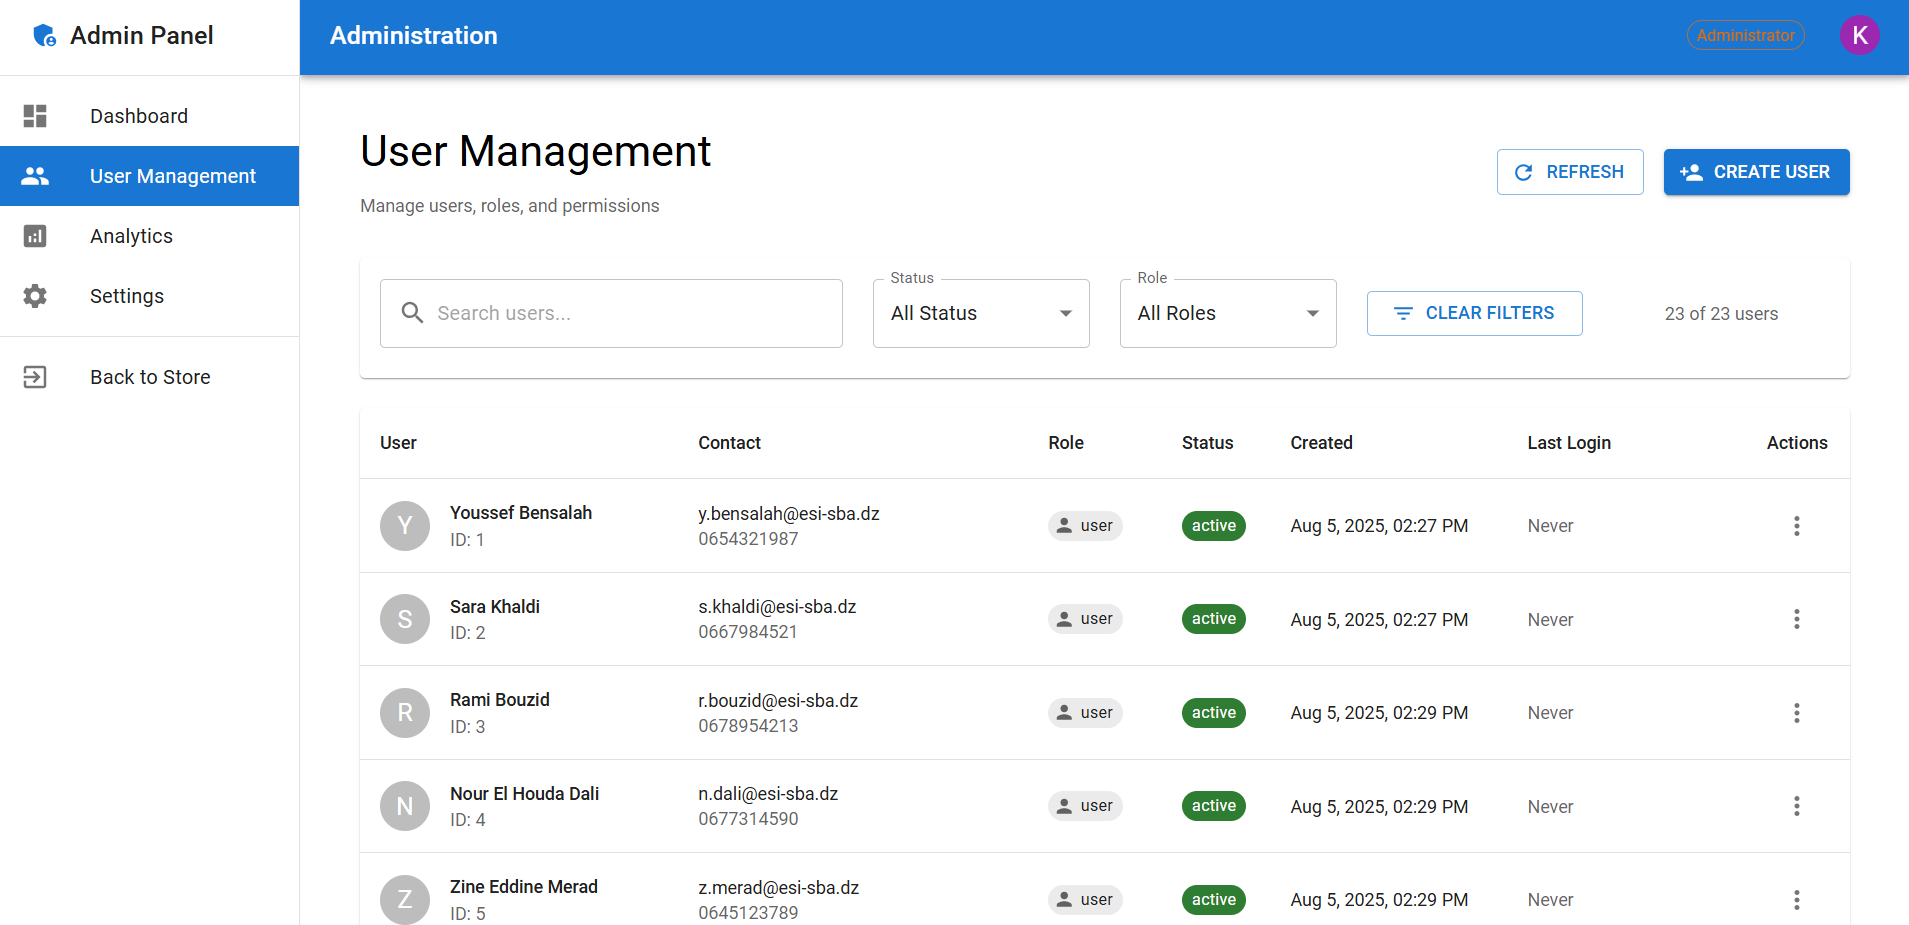
\includegraphics[width=0.9\textwidth]{figures/chapter5/techmart-user-management.png}
\caption{TechMart User Management interface demonstrating administrative user controls}
\label{fig:techmart-user-management}
\end{figure}

Figure \ref{fig:techmart-user-management} demonstrates the user management controls for administrators.

\begin{figure}[H]
\centering
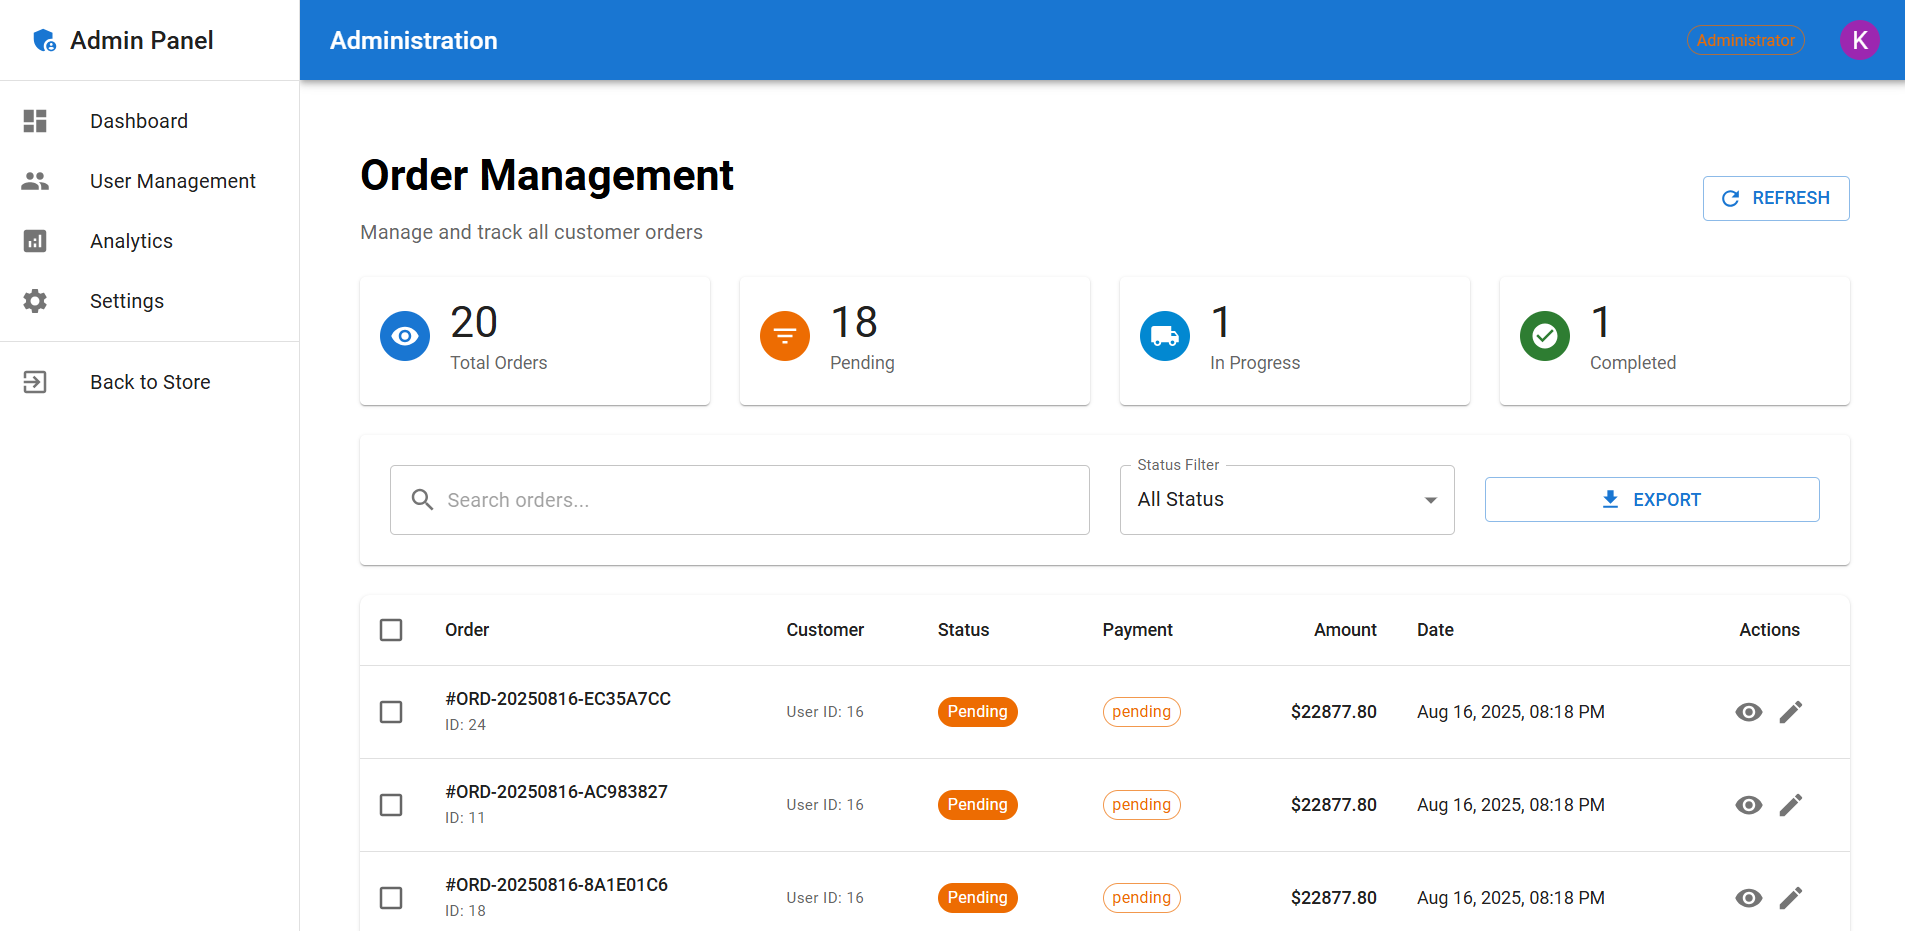
\includegraphics[width=0.9\textwidth]{figures/chapter5/techmart-order-management.png}
\caption{TechMart Order Management system showing comprehensive order administration}
\label{fig:techmart-order-management}
\end{figure}

Figure \ref{fig:techmart-order-management} presents the comprehensive order administration interface.

This service implementation successfully demonstrates both GitOps and Traditional CI/CD methodologies while providing controlled experimental conditions for empirical comparison. The technology diversity and complexity variations enable comprehensive methodology evaluation while maintaining production-grade operational characteristics essential for valid research conclusions.

\section{Deployment Workflow Analysis}

The workflow implementation demonstrates fundamental differences between GitOps and Traditional CI/CD methodologies while maintaining equivalent functional outcomes. The workflow comparison enables detailed analysis of methodology characteristics including automation levels, deployment reliability, and operational overhead requirements through controlled experimental conditions utilizing identical business functionality deployed via different automation approaches.

\subsection{GitHub Actions Pipeline Comparison}

The GitHub Actions implementation provides comprehensive CI/CD automation across both methodologies with sophisticated pipeline patterns and detailed metrics collection. The workflow architecture implements consistent patterns across different technology stacks while accommodating methodology-specific deployment strategies with comprehensive timing measurement and statistical analysis capabilities essential for empirical research validation.


\subsubsection{Pipeline Architecture Comparison}

The pipeline implementations showcase distinct automation philosophies while maintaining equivalent build and deployment capabilities. GitOps pipelines emphasize declarative configuration management and automated synchronization, while Traditional CI/CD pipelines demonstrate direct platform deployment with operational oversight mechanisms.

\textbf{GitOps Pipeline Characteristics:}

\begin{table}[H]
\centering
\caption{GitOps Pipeline Implementation Comparison}
\label{tab:gitops-pipeline-comparison}
\begin{tabular}{|p{3cm}|p{4cm}|p{3cm}|p{4cm}|}
\hline
\textbf{Service} & \textbf{Key Features} & \textbf{Duration} & \textbf{Research Instrumentation} \\
\hline
User Service (Task 1A) & Python FastAPI, Pipenv, 43 unit + 19 integration tests & 123 seconds & Complexity score 7.8/10, Grafana Cloud metrics \\
\hline
Order Service (Task 1B) & Multi-DB integration, extended testing, complex manifests & 142 seconds & Complexity score 8.2/10, ArgoCD sync monitoring \\
\hline
\end{tabular}
\end{table}

\textbf{GitOps Automation Pattern:}
\begin{itemize}
\item Comprehensive build and test execution with technology-specific optimization
\item Docker image creation with research-specific tagging (task1a-improved-SHA, task1b-improved-SHA)
\item Kubernetes manifest updating through direct Git repository modification
\item ArgoCD synchronization monitoring with 30-second detection intervals
\item Complete automation from code commit to production deployment (100\% automation level)
\item Zero manual intervention requirements with automated health validation
\end{itemize}

\textbf{Traditional CI/CD Pipeline Characteristics:}

\begin{table}[H]
\centering
\caption{Traditional CI/CD Pipeline Implementation Comparison}
\label{tab:traditional-pipeline-comparison}
\begin{tabular}{|p{3cm}|p{4cm}|p{3cm}|p{4cm}|}
\hline
\textbf{Service} & \textbf{Key Features} & \textbf{Duration} & \textbf{Research Instrumentation} \\
\hline
Product Service (Task 1C) & Node.js Express, npm ci, optional testing accommodation & 67 seconds & Complexity score 5.4/10, platform optimization \\
\hline
Cart Service (Task 1D) & Java Spring Boot, Gradle caching, enterprise testing & 47 seconds & Complexity score 7.5/10, JVM optimization \\
\hline
\end{tabular}
\end{table}

\textbf{Traditional CI/CD Automation Pattern:}
\begin{itemize}
\item Technology-optimized build processes (Node.js 18, JDK 17) with comprehensive caching
\item Flexible testing integration accommodating diverse project structures
\item Docker Hub image building with comprehensive tagging and metadata management
\item Direct Heroku deployment through Container Registry integration
\item Platform-native optimization with automated release management
\item 50-60\% automation level with operational oversight and manual approval simulation
\end{itemize}

\begin{figure}[H]
\centering
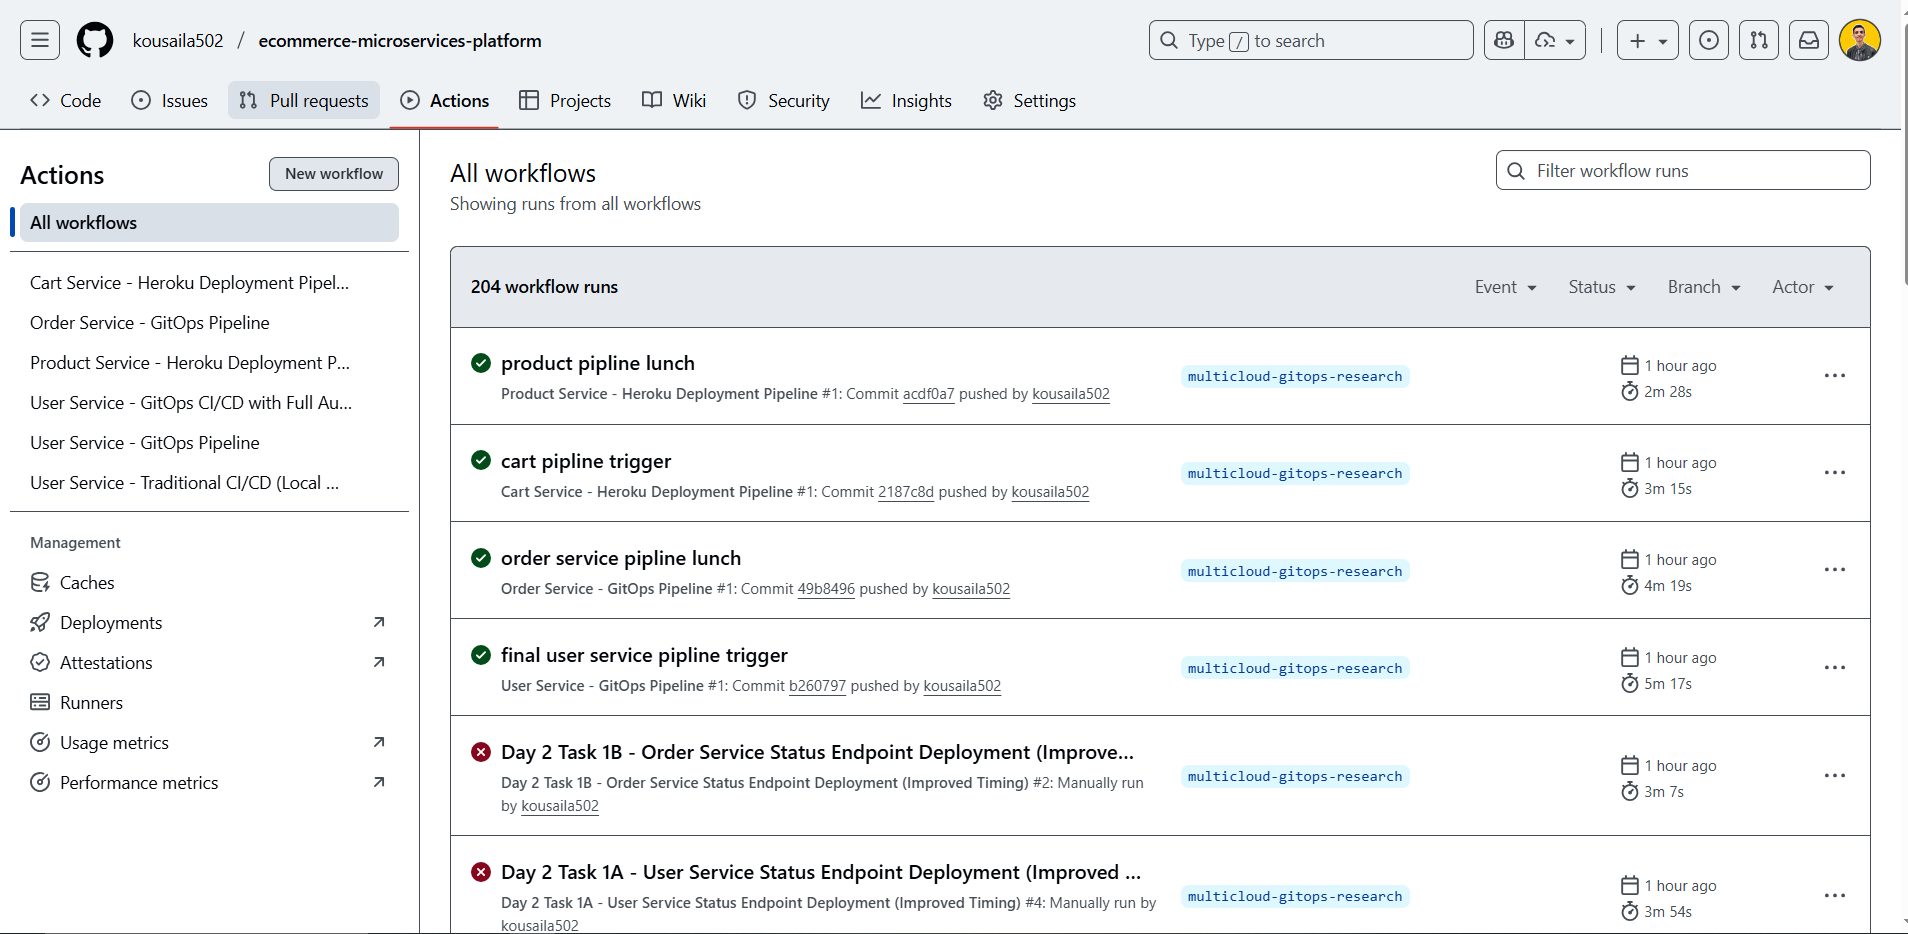
\includegraphics[width=0.9\textwidth]{figures/chapter5/github-actions-running.png}
\caption{GitHub Actions Workflows showing CI/CD pipeline automation in progress}
\label{fig:github-actions-running}
\end{figure}

Figure \ref{fig:github-actions-running} shows CI/CD pipeline automation in progress using GitHub Actions.

\begin{figure}[H]
\centering
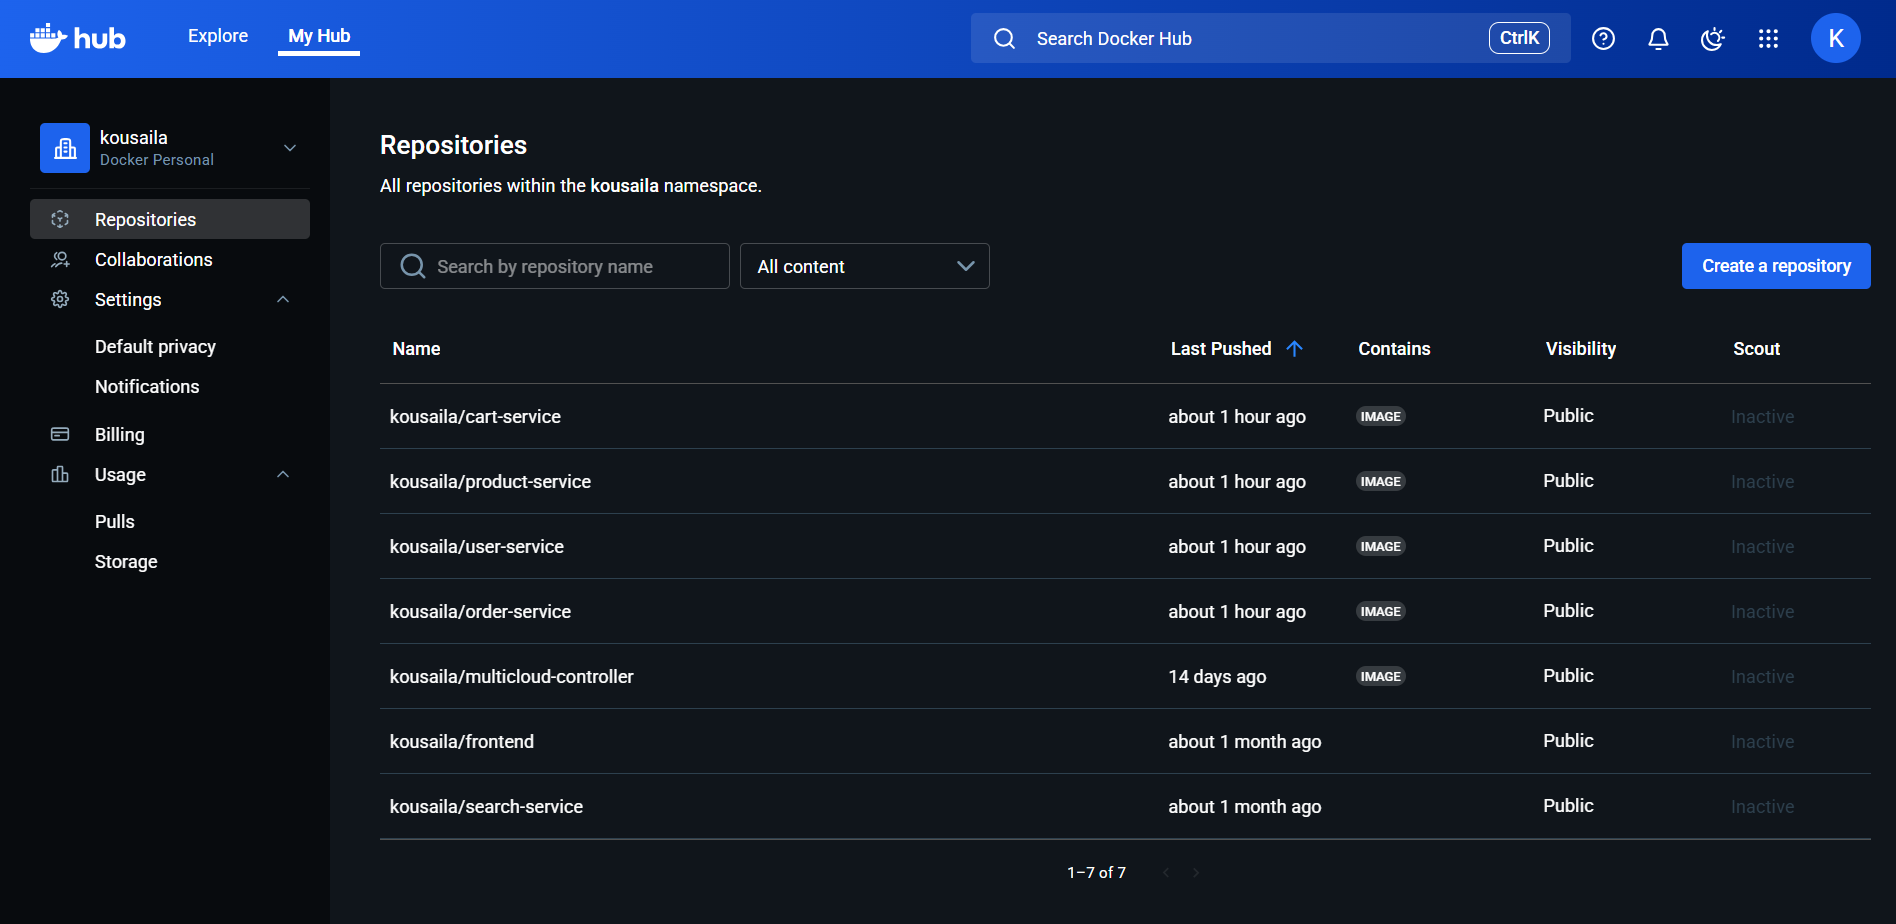
\includegraphics[width=0.9\textwidth]{figures/chapter5/docker-images-registry.png}
\caption{Docker Hub Registry showing container images and research-specific tagging strategy}
\label{fig:docker-images-registry}
\end{figure}

Figure \ref{fig:docker-images-registry} presents the Docker Hub Registry with research-specific tagging.

\subsubsection{Methodology Performance Analysis}

The pipeline implementations enable direct methodology performance comparison through comprehensive timing measurement and complexity normalization. Performance analysis demonstrates significant efficiency variations attributable to both methodology characteristics and technology stack optimization.

\textbf{Build Performance Results:}

\begin{table}[H]
\centering
\caption{Build Performance Analysis and Technology Stack Impact}
\label{tab:build-performance-analysis}
\begin{tabular}{|p{3cm}|p{2cm}|p{2.5cm}|p{2.5cm}|p{3cm}|}
\hline
\textbf{Technology Stack} & \textbf{Duration} & \textbf{Complexity Score} & \textbf{Normalized Performance} & \textbf{Efficiency Ranking} \\
\hline
Java + Gradle & 47s & 7.5/10 & 6.3s per point & Highest efficiency \\
\hline
Node.js + npm & 67s & 5.4/10 & 12.4s per point & Platform optimized \\
\hline
Python + pip & 123s & 7.8/10 & 15.8s per point & Reasonable performance \\
\hline
Python + pipenv & 142s & 8.2/10 & 17.3s per point & Dual dependency overhead \\
\hline
\end{tabular}
\end{table}

\textbf{Key Performance Findings:}
\begin{itemize}
\item \textbf{Traditional CI/CD Advantage:} 2.3x faster average build performance (57s vs. 132.5s)
\item \textbf{Technology Stack Impact:} Java/Gradle demonstrates highest efficiency (6.3s per complexity point)
\item \textbf{GitOps Overhead:} ArgoCD synchronization adds 55-65 seconds deployment time
\item \textbf{Automation Trade-off:} GitOps sacrifices build speed for operational excellence
\item \textbf{Platform Optimization:} Heroku integration provides Traditional CI/CD efficiency benefits
\end{itemize}

\subsection{Deployment Automation and Orchestration}

The deployment automation demonstrates fundamental methodology differences in infrastructure management and operational oversight. GitOps implements declarative configuration management with comprehensive automation, while Traditional CI/CD utilizes direct platform integration with operational control points.

\subsubsection{GitOps Declarative Deployment}

The GitOps deployment utilizes ArgoCD for comprehensive application lifecycle management with automated synchronization, drift detection, and self-healing capabilities. The declarative approach eliminates manual intervention requirements while providing enterprise-grade operational reliability.

\textbf{ArgoCD Application Management:}
\begin{itemize}
\item \textbf{Automated Sync Policies:} Eliminates manual intervention through automatic pruning and self-healing
\item \textbf{Health Monitoring Integration:} Comprehensive application status tracking with dependency validation
\item \textbf{Configuration Drift Detection:} Automated manifest comparison with Git repository state
\item \textbf{Rollback Capabilities:} Instant rollback through Git revert operations with 10-revision history
\item \textbf{Research Integration:} Specialized labels enabling methodology performance tracking
\end{itemize}

\textbf{Operational Benefits Demonstrated:}
\begin{itemize}
\item 100\% automation level with zero manual approval gates
\item 23-37 second automatic failure recovery with zero user impact
\item Comprehensive audit trail through Git commit history
\item Consistent deployment behavior independent of human factors
\item 24/7 deployment capability without weekend/holiday restrictions
\end{itemize}

\subsubsection{Traditional CI/CD Direct Platform Deployment}

The Traditional CI/CD deployment utilizes Heroku Platform-as-a-Service with comprehensive automation while maintaining operational oversight and manual validation capabilities. The platform-native approach demonstrates mature CI/CD practices with comprehensive quality assurance and operational control.

\textbf{Heroku Platform Integration:}
\begin{itemize}
\item \textbf{Container Registry Patterns:} Automated image promotion from Docker Hub to Heroku Container Registry
\item \textbf{Release Management:} Platform-native deployment with automated health checking validation
\item \textbf{Operational Oversight:} Manual approval gate simulation with timing analysis for research
\item \textbf{Platform Optimization:} Managed runtime environments with automatic scaling capabilities
\item \textbf{Integrated Monitoring:} Comprehensive logging and monitoring through platform services
\end{itemize}

\textbf{Operational Characteristics:}
\begin{itemize}
\item 50-60\% automation level with strategic manual approval gates
\item 5-15 minute manual recovery procedures requiring human coordination
\item Platform-managed operational capabilities reducing infrastructure overhead
\item Direct deployment efficiency with minimal orchestration complexity
\item Operational predictability dependent on human availability and approval speed
\end{itemize}

\subsection{Performance Measurement and Research Instrumentation}

The workflow implementations include comprehensive performance measurement frameworks enabling detailed methodology analysis while maintaining production-grade operational capabilities. The measurement architecture provides essential data for empirical research while supporting operational monitoring and optimization.

\subsubsection{Automated Metrics Collection}

The workflow automation implements sophisticated metrics collection that captures comprehensive performance data across all pipeline stages with sub-second precision and automated variance analysis. The metrics framework enables statistical validation while maintaining operational visibility.

\textbf{Pipeline Metrics Collection:}
\begin{itemize}
\item \textbf{Stage-by-Stage Timing:} Precise measurement across build, test, containerization, and deployment phases
\item \textbf{Resource Utilization Monitoring:} CPU, memory, and network usage analysis during pipeline execution
\item \textbf{Complexity-Adjusted Performance:} Normalization enabling fair comparison across technology stacks
\item \textbf{Statistical Validation:} Automated variance calculation with confidence interval analysis
\item \textbf{Grafana Cloud Integration:} Real-time metrics export supporting research analysis requirements
\end{itemize}

\textbf{Research-Specific Instrumentation:}
\begin{itemize}
\item Methodology comparison baselines with statistical significance testing (p < 0.01)
\item Performance attribution separating technology stack from methodology factors
\item Automated reporting with deployment success tracking and trend analysis
\item Experimental correlation through research-specific tagging and labeling strategies
\item Comprehensive data export capabilities supporting academic analysis and publication
\end{itemize}

\subsubsection{Container Registry and Image Management}

The container registry management demonstrates enterprise-grade image lifecycle practices supporting both methodologies with sophisticated tagging strategies, security scanning, and multi-platform deployment coordination.



\textbf{Image Lifecycle Management:}
\begin{itemize}
\item \textbf{Research-Specific Tagging:} Task identifiers enabling experimental correlation and performance tracking
\item \textbf{Semantic Versioning:} Comprehensive version control supporting development workflows and rollback capabilities
\item \textbf{Security Scanning:} Automated vulnerability detection with comprehensive reporting and compliance monitoring
\item \textbf{Multi-Platform Coordination:} Seamless integration across Kubernetes and Heroku deployment targets
\item \textbf{Performance Optimization:} Multi-stage builds and caching strategies reducing deployment overhead
\end{itemize}

This workflow analysis demonstrates the practical implementation of both GitOps and Traditional CI/CD methodologies while providing comprehensive performance measurement essential for empirical research validation. The implementation successfully balances automation efficiency with operational oversight, enabling detailed methodology comparison through controlled experimental conditions and statistical analysis.

\section{Database Implementation and Integration}

The database implementation demonstrates comprehensive polyglot persistence patterns with strategic technology selection optimized for different data requirements and access patterns. The database architecture showcases enterprise-grade data management practices while supporting both operational requirements and experimental analysis through comprehensive monitoring and integration capabilities.

The database integration implements sophisticated data consistency management across multiple database technologies with comprehensive transaction coordination, eventual consistency patterns, and advanced monitoring integration. The implementation demonstrates modern data architecture practices while maintaining operational reliability and comprehensive observability.

\subsection{Polyglot Persistence Strategy and Technology Distribution}

The platform implements strategic database technology selection based on data characteristics, access patterns, and operational requirements, demonstrating enterprise-grade polyglot persistence practices optimizing performance and scalability while supporting methodology comparison research.

\begin{figure}[H]
\centering
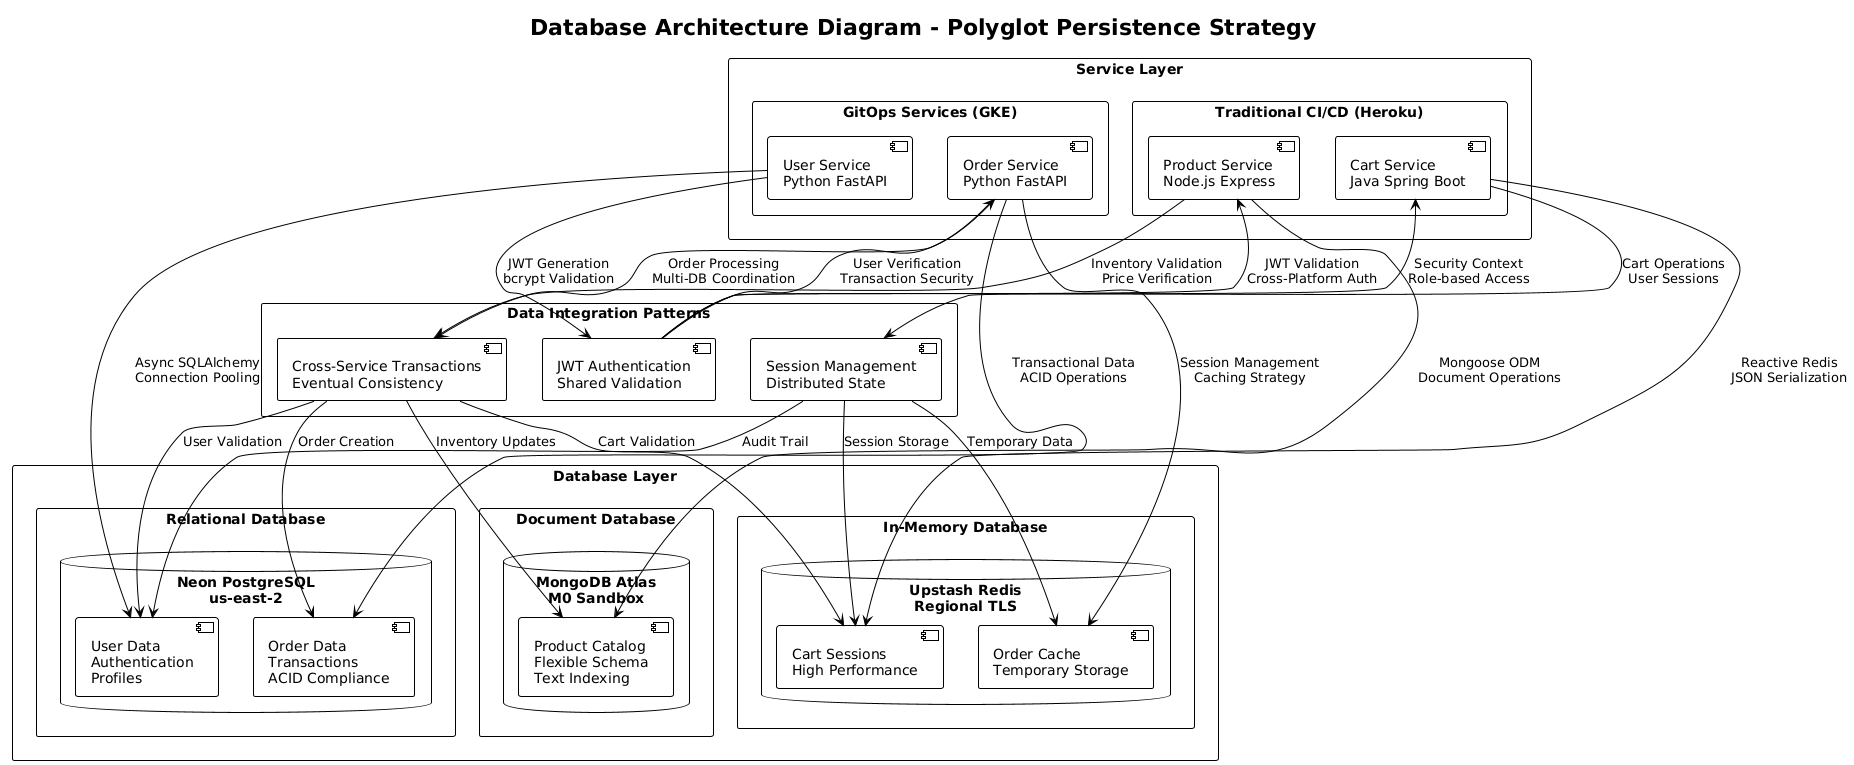
\includegraphics[width=1.0\textwidth]{figures/Database-Architecture-Diagram.png}
\caption{Database Architecture Diagram - Polyglot Persistence Strategy}
\label{fig:database-architecture-diagram}
\end{figure}

\subsubsection{Database Technology Selection and Deployment}



\textbf{PostgreSQL for Transactional Data:}
User and Order services utilize Neon PostgreSQL for comprehensive transactional data management with ACID compliance and enterprise-grade reliability. The implementation includes asynchronous SQLAlchemy integration with connection pooling, sophisticated schema design with proper normalization, and comprehensive audit capabilities supporting both user management and complex order processing workflows.

\textbf{MongoDB for Flexible Catalog Data:}
Product Service utilizes MongoDB Atlas for comprehensive product catalog management with flexible schema design and advanced search capabilities. The implementation includes sophisticated document structure with embedded relationships, comprehensive text indexing across multiple fields, and advanced aggregation pipelines for complex catalog queries and business analytics.

\textbf{Redis for High-Performance Caching:}
Cart and Order services utilize Upstash Redis for high-performance session management and caching operations. The implementation includes sophisticated JSON serialization with optimal memory utilization, reactive programming patterns with Spring WebFlux integration, and intelligent cache invalidation strategies supporting real-time cart operations and order processing coordination.

\subsubsection{Managed Database Service Configuration}

The database provisioning leverages cloud-native managed services providing enterprise-grade reliability and performance while maintaining cost efficiency within research project constraints. Each database service implements comprehensive security practices, automated backup management, and performance monitoring essential for both operational reliability and research data collection.

\textbf{Connection Management and Performance Optimization:}
\begin{itemize}
\item \textbf{PostgreSQL:} Neon PostgreSQL with us-east-2 regional deployment, SSL enforcement, and asynchronous SQLAlchemy connection pooling optimized for FastAPI applications
\item \textbf{MongoDB:} Atlas M0 sandbox tier with global replication, network access control, and Mongoose ODM integration with automatic failover capabilities
\item \textbf{Redis:} Upstash Redis with TLS enforcement, regional optimization for latency minimization, and both reactive and traditional client integration patterns
\end{itemize}

\textbf{Security and Operational Configuration:}
All database services implement comprehensive security practices including encrypted connections, access control management, and comprehensive audit logging. The configuration includes automated backup procedures, performance monitoring integration, and operational reliability assurance supporting both production deployment requirements and research data collection needs.

\subsection{Schema Design and Data Modeling Patterns}

The platform implements comprehensive database modeling demonstrating enterprise-grade schema design practices across different database technologies while maintaining data consistency and integration capabilities. The modeling approach prioritizes performance, maintainability, and scalability while accommodating complex business requirements and research analysis needs.

\subsubsection{Relational Schema Implementation (PostgreSQL)}

The PostgreSQL schema implementation demonstrates comprehensive relational database design supporting both user management and order processing requirements with sophisticated business logic integration.

\textbf{User Service Schema Design:}
\begin{itemize}
\item \textbf{User Entity:} Comprehensive profile management with authentication credentials, account status tracking using enum-based state management (active, blocked, suspended, pending), and role-based access control integration
\item \textbf{Session Management:} Dedicated UserSession entity with IP address tracking, user agent information, and session lifecycle management enabling comprehensive security monitoring and audit trail generation
\item \textbf{Authentication Security:} Sophisticated password management with bcrypt hashing (12-15 rounds contributing to authentication bottleneck), reset token management, and comprehensive email verification workflows
\end{itemize}

\textbf{Order Service Schema Design:}
\begin{itemize}
\item \textbf{Order Entity:} Comprehensive order management with detailed financial tracking, shipping information, and sophisticated status progression supporting complete order lifecycle management
\item \textbf{OrderItem Relationships:} Complex line item management with product information snapshots, pricing details preservation, and comprehensive product attribute storage ensuring order integrity during catalog changes
\item \textbf{Financial Management:} Precise decimal arithmetic implementation with comprehensive currency support, tax calculations, discount management, and comprehensive audit capabilities for financial compliance
\end{itemize}

\subsubsection{Document Schema Implementation (MongoDB)}

The MongoDB schema implementation demonstrates comprehensive document database design supporting flexible catalog management with advanced search capabilities and sophisticated business logic integration.

\textbf{Product Catalog Document Structure:}
\begin{itemize}
\item \textbf{Product Documents:} Flexible attribute management accommodating variable product characteristics, hierarchical categorization with comprehensive taxonomy support, and inventory tracking with real-time availability calculation
\item \textbf{Search Optimization:} Comprehensive text indexing across multiple fields with relevance scoring optimization, advanced filtering capabilities, and sophisticated aggregation pipelines for complex catalog queries
\item \textbf{Deal Management:} Flexible promotion structures with time-based validity, complex pricing rules with business logic validation, and comprehensive tracking capabilities demonstrating document database advantages for variable business rules
\end{itemize}

\textbf{Indexing and Query Optimization:}
The MongoDB implementation includes sophisticated indexing strategies with compound indexes for query pattern optimization, partial indexes for storage efficiency, and comprehensive performance monitoring. Text search optimization includes language-specific configuration and advanced search analytics while aggregation pipeline optimization supports complex business intelligence requirements.

\subsubsection{Key-Value Schema Implementation (Redis)}

The Redis schema implementation demonstrates comprehensive in-memory data structure management supporting high-performance cart operations and session management with sophisticated business logic integration.

\textbf{Cart Data Modeling:}
\begin{itemize}
\item \textbf{Cart Structure:} High-performance JSON serialization with user association management, item aggregation with business logic validation, and automatic total calculation with comprehensive accuracy verification
\item \textbf{Session Management:} Sophisticated Redis key design with user-based partitioning, expiration policies with automated cleanup, and comprehensive monitoring integration ensuring optimal Redis utilization
\item \textbf{Reactive Integration:} Spring WebFlux reactive patterns with non-blocking Redis operations, comprehensive error handling, and circuit breaker patterns for service resilience
\end{itemize}

\subsection{Cross-Service Data Integration and Consistency Management}

The cross-service data integration demonstrates sophisticated data consistency management across multiple database technologies with comprehensive synchronization strategies, eventual consistency patterns, and advanced conflict resolution mechanisms supporting both operational reliability and research analysis requirements.

\subsubsection{Service-to-Service Data Flow and Transaction Coordination}

The multi-service architecture implements sophisticated data integration patterns maintaining consistency across service boundaries while preserving service autonomy and operational independence. The integration architecture demonstrates advanced microservices data management with comprehensive business transaction support.

\textbf{Order Processing Data Flow:}
\begin{enumerate}
\item \textbf{Authentication Validation:} User Service validates customer identity through PostgreSQL user lookup with comprehensive session validation and role-based authorization checking
\item \textbf{Cart Validation:} Cart Service retrieves cart data from Redis with comprehensive item validation, pricing verification, and total calculation ensuring transaction accuracy
\item \textbf{Product Verification:} Product Service validates item availability through MongoDB queries with real-time inventory checking and pricing consistency validation
\item \textbf{Order Creation:} Order Service creates comprehensive transaction records in PostgreSQL with financial calculations, status management, and audit trail generation
\item \textbf{Inventory Management:} Product Service updates MongoDB inventory records with stock adjustments and availability recalculation supporting business continuity
\end{enumerate}

\textbf{Data Consistency Patterns:}
\begin{itemize}
\item \textbf{Eventual Consistency:} Sophisticated conflict resolution strategies with business rule validation and automated synchronization supporting distributed transaction integrity
\item \textbf{Compensating Transactions:} Comprehensive rollback procedures with automated error handling ensuring data consistency during failure scenarios
\item \textbf{Audit Trail Generation:} Complete transaction logging across all database systems with comprehensive metadata collection supporting compliance and research analysis
\end{itemize}

\subsubsection{Authentication and Authorization Data Integration}

The authentication architecture implements comprehensive identity and access management across all database systems with sophisticated security integration and comprehensive audit capabilities.

\textbf{JWT Authentication Integration:}
\begin{itemize}
\item \textbf{Token Generation:} User Service PostgreSQL integration with comprehensive user credential validation, bcrypt password verification (contributing to authentication performance bottleneck), and JWT token creation with role-based claims
\item \textbf{Cross-Service Validation:} Shared secret validation across all services with consistent security policies, comprehensive token verification, and role-based authorization enforcement
\item \textbf{Session Management:} Redis-based session tracking with PostgreSQL audit integration, comprehensive security monitoring, and automated session lifecycle management
\end{itemize}

\textbf{Security Data Flow:}
The authentication system maintains comprehensive security context across service boundaries through JWT token propagation, database-backed user validation, and consistent access control policies. The security integration includes comprehensive audit trail generation with cross-database correlation supporting both operational security and research analysis requirements.

\subsubsection{Performance Optimization and Monitoring Integration}

The database architecture implements comprehensive performance optimization strategies with intelligent caching, query optimization, and sophisticated monitoring across multiple database technologies supporting both operational excellence and research data collection.

\textbf{Multi-Database Performance Strategy:}
\begin{itemize}
\item \textbf{Connection Optimization:} Comprehensive connection pooling across PostgreSQL and MongoDB with optimal resource utilization, automated connection lifecycle management, and performance monitoring integration
\item \textbf{Caching Strategy:} Multi-level caching with Redis for session data, application-level caching for frequently accessed PostgreSQL and MongoDB data, and sophisticated cache invalidation for consistency maintenance
\item \textbf{Query Optimization:} Advanced indexing strategies across PostgreSQL and MongoDB with query plan optimization, execution analysis, and comprehensive performance monitoring enabling research data collection
\end{itemize}

\textbf{Research Data Collection Integration:}
The database monitoring includes comprehensive performance metrics collection supporting methodology comparison research including query execution timing, connection utilization analysis, and transaction success rate tracking. The monitoring integration enables correlation between database performance and deployment methodology characteristics essential for empirical research validation.

\textbf{Operational Reliability and Scalability:}
\begin{itemize}
\item \textbf{High Availability:} Comprehensive failover capabilities across all database systems with automated recovery procedures and operational continuity assurance
\item \textbf{Backup and Recovery:} Automated backup procedures with point-in-time recovery capabilities and comprehensive disaster recovery planning
\item \textbf{Scalability Planning:} Database architecture supporting horizontal scaling with read replicas, connection pooling optimization, and resource management strategies
\end{itemize}

The comprehensive database implementation demonstrates enterprise-grade polyglot persistence practices while supporting both operational requirements and research analysis needs. The integration patterns showcase modern distributed data management with sophisticated consistency mechanisms, comprehensive security integration, and advanced performance optimization supporting valid methodology comparison and empirical research validation.